% !TeX spellcheck = hu_HU
% !TeX encoding = UTF-8
% !TeX program = xelatex
\documentclass[11pt,a4paper,oneside]{report}             % Single-side
%\documentclass[11pt,a4paper,twoside,openright]{report}  % Duplex

% thanks to http://tex.stackexchange.com/a/47579/71109
\usepackage{ifxetex}
\usepackage{ifluatex}
\newif\ifxetexorluatex % a new conditional starts as false
\ifnum 0\ifxetex 1\fi\ifluatex 1\fi>0
   \xetexorluatextrue
\fi

\ifxetexorluatex
  \usepackage{fontspec}
\else
  \usepackage[T1]{fontenc}
  \usepackage[utf8]{inputenc}
  \usepackage[lighttt]{lmodern}
\fi

\usepackage[english,magyar]{babel} % Alapértelmezés szerint utoljára definiált nyelv lesz aktív, de később külön beállítjuk az aktív nyelvet.

%\usepackage{cmap}
\usepackage{amsfonts,amsmath,amssymb} % Mathematical symbols.
%\usepackage[ruled,boxed,resetcount,linesnumbered]{algorithm2e} % For pseudocodes. % beware: this is not compatible with LuaLaTeX, see http://tex.stackexchange.com/questions/34814/lualatex-and-algorithm2e
\usepackage{booktabs} % For publication quality tables for LaTeX
\usepackage{graphicx}

%\usepackage{fancyhdr}
%\usepackage{lastpage}

\usepackage{anysize}
%\usepackage{sectsty}
\usepackage{setspace} % For setting line spacing

\usepackage[unicode]{hyperref} % For hyperlinks in the generated document.
\usepackage{xcolor}
\usepackage{listings} % For source code snippets.

\usepackage[amsmath,thmmarks]{ntheorem} % Theorem-like environments.

\usepackage[hang]{caption}

\singlespacing

\newcommand{\selecthungarian}{
	\selectlanguage{magyar}
	\setlength{\parindent}{2em}
	\setlength{\parskip}{0em}
	\frenchspacing
}

\newcommand{\selectenglish}{
	\selectlanguage{english}
	\setlength{\parindent}{0em}
	\setlength{\parskip}{0.5em}
	\nonfrenchspacing
	\renewcommand{\figureautorefname}{Figure}
	\renewcommand{\tableautorefname}{Table}
	\renewcommand{\partautorefname}{Part}
	\renewcommand{\chapterautorefname}{Chapter}
	\renewcommand{\sectionautorefname}{Section}
	\renewcommand{\subsectionautorefname}{Section}
	\renewcommand{\subsubsectionautorefname}{Section}
}

\usepackage[numbers]{natbib}
\usepackage{xspace}


\newcommand{\vikszerzoVezeteknev}{Nánási}
\newcommand{\vikszerzoKeresztnev}{Dániel}

\newcommand{\vikkonzulensAMegszolitas}{Dr. }
\newcommand{\vikkonzulensAVezeteknev}{Simon}
\newcommand{\vikkonzulensAKeresztnev}{Csaba}

\newcommand{\vikkonzulensBMegszolitas}{}
\newcommand{\vikkonzulensBVezeteknev}{}
\newcommand{\vikkonzulensBKeresztnev}{}

\newcommand{\vikkonzulensCMegszolitas}{}
\newcommand{\vikkonzulensCVezeteknev}{}
\newcommand{\vikkonzulensCKeresztnev}{}

\newcommand{\vikcim}{Felhő alapú drónvezérlés} % Cím
\newcommand{\viktanszek}{\bmetmit} % Tanszék
\newcommand{\vikdoktipus}{\msc} % Dokumentum típusa (\bsc vagy \msc)
\newcommand{\vikmunkatipusat}{diplomatervet} % a "hallgató nyilatkozat" részhez: szakdolgozatot vagy diplomatervet

%--------------------------------------------------------------------------------------
% TDK-specifikus változók
%--------------------------------------------------------------------------------------
\newcommand{\tdkszerzoB}{Második Szerző} % Második szerző neve; hagyd üresen, ha egyedül írtad a TDK-t.
\newcommand{\tdkev}{2014} % A dolgozat írásának éve (pl. "2014") (Ez OTDK-nál eltérhet az aktuális évtől.)

% További adatok az OTDK címlaphoz (BME-s TDK-hoz nem kell kitölteni)
\newcommand{\tdkevfolyamA}{IV} % Első szerző évfolyama, római számmal (pl. IV).
\newcommand{\tdkevfolyamB}{III} % Második szerző évfolyama, római számmal (pl. III).
\newcommand{\tdkkonzulensbeosztasA}{egyetemi tanár} % Első konzulens beosztása (pl. egyetemi docens)
\newcommand{\tdkkonzulensbeosztasB}{doktorandusz} % Második konzulens beosztása (pl. egyetemi docens)

\newcommand{\szerzoMeta}{\vikszerzoVezeteknev{} \vikszerzoKeresztnev} % egy szerző esetén
%\newcommand{\szerzoMeta}{\vikszerzoVezeteknev{} \vikszerzoKeresztnev, \tdkszerzoB} % két szerző esetén

% Beállítások magyar nyelvű dolgozathoz
%%--------------------------------------------------------------------------------------
% Elnevezések
%--------------------------------------------------------------------------------------
\newcommand{\bme}{Budapesti Műszaki és Gazdaságtudományi Egyetem}
\newcommand{\vik}{Villamosmérnöki és Informatikai Kar}

\newcommand{\bmemit}{Méréstechnika és Információs Rendszerek Tanszék}
\newcommand{\bmetmit}{Távközlési és Médiainformatikai Tanszék}

\newcommand{\keszitette}{Készítette}
\newcommand{\konzulens}{Konzulens}

\newcommand{\bsc}{Szakdolgozat}
\newcommand{\msc}{Diplomaterv}
\newcommand{\tdk}{TDK dolgozat}
\newcommand{\bsconlab}{BSc Önálló laboratórium}
\newcommand{\msconlabi}{MSc Önálló laboratórium 1.}
\newcommand{\msconlabii}{MSc Önálló laboratórium 2.}

\newcommand{\pelda}{Példa}
\newcommand{\definicio}{Definíció}
\newcommand{\tetel}{Tétel}

\newcommand{\bevezetes}{Bevezetés}
\newcommand{\koszonetnyilvanitas}{Köszönetnyilvánítás}
\newcommand{\fuggelek}{Függelék}

% Opcionálisan átnevezhető címek
%\addto\captionsmagyar{%
%\renewcommand{\listfigurename}{Saját ábrajegyzék cím}
%\renewcommand{\listtablename}{Saját táblázatjegyzék cím}
%\renewcommand{\bibname}{Saját irodalomjegyzék név}
%}


\newcommand{\szerzo}{\vikszerzoVezeteknev{} \vikszerzoKeresztnev}
\newcommand{\vikkonzulensA}{\vikkonzulensAMegszolitas\vikkonzulensAVezeteknev{} \vikkonzulensAKeresztnev}
\newcommand{\vikkonzulensB}{\vikkonzulensBMegszolitas\vikkonzulensBVezeteknev{} \vikkonzulensBKeresztnev}
\newcommand{\vikkonzulensC}{\vikkonzulensCMegszolitas\vikkonzulensCVezeteknev{} \vikkonzulensCKeresztnev}

\newcommand{\selectthesislanguage}{\selecthungarian}

\bibliographystyle{huplain}

\def\lstlistingname{lista}

\newcommand{\appendixnumber}{6}  % a fofejezet-szamlalo az angol ABC 6. betuje (F) lesz

% Settings for English documents
%--------------------------------------------------------------------------------------
% Elnevezések
%--------------------------------------------------------------------------------------
\newcommand{\bme}{Budapesti Műszaki és Gazdaságtudományi Egyetem}
\newcommand{\vik}{Villamosmérnöki és Informatikai Kar}

\newcommand{\bmemit}{Méréstechnika és Információs Rendszerek Tanszék}
\newcommand{\bmetmit}{Távközlési és Médiainformatikai Tanszék}

\newcommand{\keszitette}{Készítette}
\newcommand{\konzulens}{Konzulens}

\newcommand{\bsc}{Szakdolgozat}
\newcommand{\msc}{Diplomaterv}
\newcommand{\tdk}{TDK dolgozat}
\newcommand{\bsconlab}{BSc Önálló laboratórium}
\newcommand{\msconlabi}{MSc Önálló laboratórium 1.}
\newcommand{\msconlabii}{MSc Önálló laboratórium 2.}

\newcommand{\pelda}{Példa}
\newcommand{\definicio}{Definíció}
\newcommand{\tetel}{Tétel}

\newcommand{\bevezetes}{Bevezetés}
\newcommand{\koszonetnyilvanitas}{Köszönetnyilvánítás}
\newcommand{\fuggelek}{Függelék}

% Opcionálisan átnevezhető címek
%\addto\captionsmagyar{%
%\renewcommand{\listfigurename}{Saját ábrajegyzék cím}
%\renewcommand{\listtablename}{Saját táblázatjegyzék cím}
%\renewcommand{\bibname}{Saját irodalomjegyzék név}
%}


\newcommand{\szerzo}{\vikszerzoVezeteknev{} \vikszerzoKeresztnev}
\newcommand{\vikkonzulensA}{\vikkonzulensAMegszolitas\vikkonzulensAVezeteknev{} \vikkonzulensAKeresztnev}
\newcommand{\vikkonzulensB}{\vikkonzulensBMegszolitas\vikkonzulensBVezeteknev{} \vikkonzulensBKeresztnev}
\newcommand{\vikkonzulensC}{\vikkonzulensCMegszolitas\vikkonzulensCVezeteknev{} \vikkonzulensCKeresztnev}

\newcommand{\selectthesislanguage}{\selecthungarian}

\bibliographystyle{huplain}

\def\lstlistingname{lista}

\newcommand{\appendixnumber}{6}  % a fofejezet-szamlalo az angol ABC 6. betuje (F) lesz

%--------------------------------------------------------------------------------------
% Page layout setup
%--------------------------------------------------------------------------------------
% we need to redefine the pagestyle plain
% another possibility is to use the body of this command without \fancypagestyle
% and use \pagestyle{fancy} but in that case the special pages
% (like the ToC, the References, and the Chapter pages)remain in plane style

\pagestyle{plain}
\marginsize{35mm}{25mm}{15mm}{15mm}

\setcounter{tocdepth}{3}
%\sectionfont{\large\upshape\bfseries}
\setcounter{secnumdepth}{3}

\sloppy % Margón túllógó sorok tiltása.
\widowpenalty=10000 \clubpenalty=10000 %A fattyú- és árvasorok elkerülése
\def\hyph{-\penalty0\hskip0pt\relax} % Kötőjeles szavak elválasztásának engedélyezése


%--------------------------------------------------------------------------------------
% Setup hyperref package
%--------------------------------------------------------------------------------------
\hypersetup{
    % bookmarks=true,            % show bookmarks bar?
    unicode=true,              % non-Latin characters in Acrobat's bookmarks
    pdftitle={\vikcim},        % title
    pdfauthor={\szerzoMeta},    % author
    pdfsubject={\vikdoktipus}, % subject of the document
    pdfcreator={\szerzoMeta},   % creator of the document
    pdfproducer={},    % producer of the document
    pdfkeywords={},    % list of keywords (separate then by comma)
    pdfnewwindow=true,         % links in new window
    colorlinks=true,           % false: boxed links; true: colored links
    linkcolor=black,           % color of internal links
    citecolor=black,           % color of links to bibliography
    filecolor=black,           % color of file links
    urlcolor=black             % color of external links
}


%--------------------------------------------------------------------------------------
% Set up listings
%--------------------------------------------------------------------------------------
\definecolor{lightgray}{rgb}{0.95,0.95,0.95}
\lstset{
	basicstyle=\scriptsize\ttfamily, % print whole listing small
	keywordstyle=\color{black}\bfseries, % bold black keywords
	identifierstyle=, % nothing happens
	% default behavior: comments in italic, to change use
	% commentstyle=\color{green}, % for e.g. green comments
	stringstyle=\scriptsize,
	showstringspaces=false, % no special string spaces
	aboveskip=3pt,
	belowskip=3pt,
	backgroundcolor=\color{lightgray},
	columns=flexible,
	keepspaces=true,
	escapeinside={(*@}{@*)},
	captionpos=b,
	breaklines=true,
	frame=single,
	float=!ht,
	tabsize=2,
	literate=*
		{á}{{\'a}}1	{é}{{\'e}}1	{í}{{\'i}}1	{ó}{{\'o}}1	{ö}{{\"o}}1	{ő}{{\H{o}}}1	{ú}{{\'u}}1	{ü}{{\"u}}1	{ű}{{\H{u}}}1
		{Á}{{\'A}}1	{É}{{\'E}}1	{Í}{{\'I}}1	{Ó}{{\'O}}1	{Ö}{{\"O}}1	{Ő}{{\H{O}}}1	{Ú}{{\'U}}1	{Ü}{{\"U}}1	{Ű}{{\H{U}}}1
}


%--------------------------------------------------------------------------------------
% Set up theorem-like environments
%--------------------------------------------------------------------------------------
% Using ntheorem package -- see http://www.math.washington.edu/tex-archive/macros/latex/contrib/ntheorem/ntheorem.pdf

\theoremstyle{plain}
\theoremseparator{.}
\newtheorem{example}{\pelda}

\theoremseparator{.}
%\theoremprework{\bigskip\hrule\medskip}
%\theorempostwork{\hrule\bigskip}
\theorembodyfont{\upshape}
\theoremsymbol{{\large \ensuremath{\centerdot}}}
\newtheorem{definition}{\definicio}

\theoremseparator{.}
%\theoremprework{\bigskip\hrule\medskip}
%\theorempostwork{\hrule\bigskip}
\newtheorem{theorem}{\tetel}


%--------------------------------------------------------------------------------------
% Some new commands and declarations
%--------------------------------------------------------------------------------------
\newcommand{\code}[1]{{\upshape\ttfamily\scriptsize\indent #1}}
\newcommand{\doi}[1]{DOI: \href{http://dx.doi.org/\detokenize{#1}}{\raggedright{\texttt{\detokenize{#1}}}}} % A hivatkozások közt így könnyebb DOI-t megadni.

\DeclareMathOperator*{\argmax}{arg\,max}
%\DeclareMathOperator*[1]{\floor}{arg\,max}
\DeclareMathOperator{\sign}{sgn}
\DeclareMathOperator{\rot}{rot}


%--------------------------------------------------------------------------------------
% Setup captions
%--------------------------------------------------------------------------------------
\captionsetup[figure]{
	width=.75\textwidth,
	aboveskip=10pt}

\renewcommand{\captionlabelfont}{\bf}
%\renewcommand{\captionfont}{\footnotesize\it}

%--------------------------------------------------------------------------------------
% Hyphenation exceptions
%--------------------------------------------------------------------------------------
\hyphenation{Shakes-peare Mar-seilles ár-víz-tű-rő tü-kör-fú-ró-gép}


\author{\vikszerzo}
\title{\viktitle}

% saját beállítások

% enter paragraph után
\newcommand{\paragraphl}[1]{\paragraph{#1}\mbox{}\\} 

\renewcommand\lstlistlistingname{Listák jegyzéke}

% pipa és x
\usepackage{amssymb}% http://ctan.org/pkg/amssymb
\usepackage{pifont}% http://ctan.org/pkg/pifont
\newcommand{\cmark}{\ding{51}}%
\newcommand{\xmark}{\ding{55}}%

\lstdefinestyle{yamlCode} {
	numbers=left,
	language=Yaml,
	backgroundcolor={\color{lightgray!40}},
	breaklines=true,
	frame=single,
	columns=fixed
}

\renewcommand{\lstlistingname}{kódrészlet}% Listing -> Algorithm
\renewcommand{\lstlistlistingname}{Kódrészletek jegyzéke}% List of Listings -> List of Algorithms

%--------------------------------------------------------------------------------------
% Table of contents and the main text
%--------------------------------------------------------------------------------------
\begin{document}
%\pagenumbering{arabic}
\pagenumbering{gobble}

%~~~~~~~~~~~~~~~~~~~~~~~~~~~~~~~~~~~~~~~~~~~~~~~~~~~~~~~~~~~~~~~~~~~~~~~~~~~~~~~~~~~~~~
%\selecthungarian
%--------------------------------------------------------------------------------------
% Rovid formai es tartalmi tajekoztato
%--------------------------------------------------------------------------------------

\footnotesize
\begin{center}
\large
\textbf{\Large Általános információk, a diplomaterv szerkezete}\\
\end{center}

A diplomaterv szerkezete a BME Villamosmérnöki és Informatikai Karán:
\begin{enumerate}
\item	Diplomaterv feladatkiírás
\item	Címoldal
\item	Tartalomjegyzék
\item	A diplomatervező nyilatkozata az önálló munkáról és az elektronikus adatok kezeléséről
\item	Tartalmi összefoglaló magyarul és angolul
\item	Bevezetés: a feladat értelmezése, a tervezés célja, a feladat indokoltsága, a diplomaterv felépítésének rövid összefoglalása
\item	A feladatkiírás pontosítása és részletes elemzése
\item	Előzmények (irodalomkutatás, hasonló alkotások), az ezekből levonható következtetések
\item	A tervezés részletes leírása, a döntési lehetőségek értékelése és a választott megoldások indoklása
\item	A megtervezett műszaki alkotás értékelése, kritikai elemzése, továbbfejlesztési lehetőségek
\item	Esetleges köszönetnyilvánítások
\item	Részletes és pontos irodalomjegyzék
\item	Függelék(ek)
\end{enumerate}

Felhasználható a következő oldaltól kezdődő \LaTeX diplomatervsablon dokumentum tartalma. 

A diplomaterv szabványos méretű A4-es lapokra kerüljön. Az oldalak tükörmargóval készüljenek (mindenhol 2,5~cm, baloldalon 1~cm-es kötéssel). Az alapértelmezett betűkészlet a 12 pontos Times New Roman, másfeles sorközzel, de ettől kismértékben el lehet térni, ill. más betűtípus használata is megengedett.

Minden oldalon -- az első négy szerkezeti elem kivételével -- szerepelnie kell az oldalszámnak.

A fejezeteket decimális beosztással kell ellátni. Az ábrákat a megfelelő helyre be kell illeszteni, fejezetenként decimális számmal és kifejező címmel kell ellátni. A fejezeteket decimális aláosztással számozzuk, maximálisan 3 aláosztás mélységben (pl. 2.3.4.1.). Az ábrákat, táblázatokat és képleteket célszerű fejezetenként külön számozni (pl. 2.4. ábra, 4.2. táblázat vagy képletnél (3.2)). A fejezetcímeket igazítsuk balra, a normál szövegnél viszont használjunk sorkiegyenlítést. Az ábrákat, táblázatokat és a hozzájuk tartozó címet igazítsuk középre. A cím a jelölt rész alatt helyezkedjen el.

A képeket lehetőleg rajzoló programmal készítsék el, az egyenleteket egyenlet-szerkesztő segítségével írják le (A \LaTeX~ehhez kézenfekvő megoldásokat nyújt).

Az irodalomjegyzék szövegközi hivatkozása történhet sorszámozva (ez a preferált megoldás) vagy a Harvard-rendszerben (a szerző és az évszám megadásával). A teljes lista névsor szerinti sorrendben a szöveg végén szerepeljen (sorszámozott irodalmi hivatkozások esetén hivatkozási sorrendben). A szakirodalmi források címeit azonban mindig az eredeti nyelven kell megadni, esetleg zárójelben a fordítással. A listában szereplő valamennyi publikációra hivatkozni kell a szövegben (a \LaTeX-sablon a Bib\TeX~segítségével mindezt automatikusan kezeli). Minden publikáció a szerzők után a következő adatok szerepelnek: folyóirat cikkeknél a pontos cím, a folyóirat címe, évfolyam, szám, oldalszám tól-ig. A folyóiratok címét csak akkor rövidítsük, ha azok nagyon közismertek vagy nagyon hosszúak. Internetes hivatkozások megadásakor fontos, hogy az elérési út előtt megadjuk az oldal tulajdonosát és tartalmát (mivel a link egy idő után akár elérhetetlenné is válhat), valamint az elérés időpontját.

\vspace{5mm}
Fontos:
\begin{itemize}
	\item A szakdolgozatkészítő / diplomatervező nyilatkozata (a jelen sablonban szereplő szövegtartalommal) kötelező előírás, Karunkon ennek hiányában a szakdolgozat/diplomaterv nem bírálható és nem védhető!
	\item Mind a dolgozat, mind a melléklet maximálisan 15~MB méretű lehet!
\end{itemize}

\vspace{5mm}
\begin{center}
Jó munkát, sikeres szakdolgozatkészítést, ill. diplomatervezést kívánunk!
\end{center}

\normalsize
\selectthesislanguage

%%--------------------------------------------------------------------------------------
% Feladatkiiras (a tanszeken atveheto, kinyomtatott valtozat)
%--------------------------------------------------------------------------------------
\clearpage
\begin{center}
\large
\textbf{FELADATKIÍRÁS}\\
\end{center}

A feladatkiírást a tanszéki adminisztrációban lehet átvenni, és a leadott munkába eredeti, tanszéki pecséttel ellátott és a tanszékvezető által aláírt lapot kell belefűzni (ezen oldal \emph{helyett}, ez az oldal csak útmutatás). Az elektronikusan feltöltött dolgozatban már nem kell beleszerkeszteni ezt a feladatkiírást.

%feladatkiírás, majd az eredeti aláírtat kell hozzáfűzni
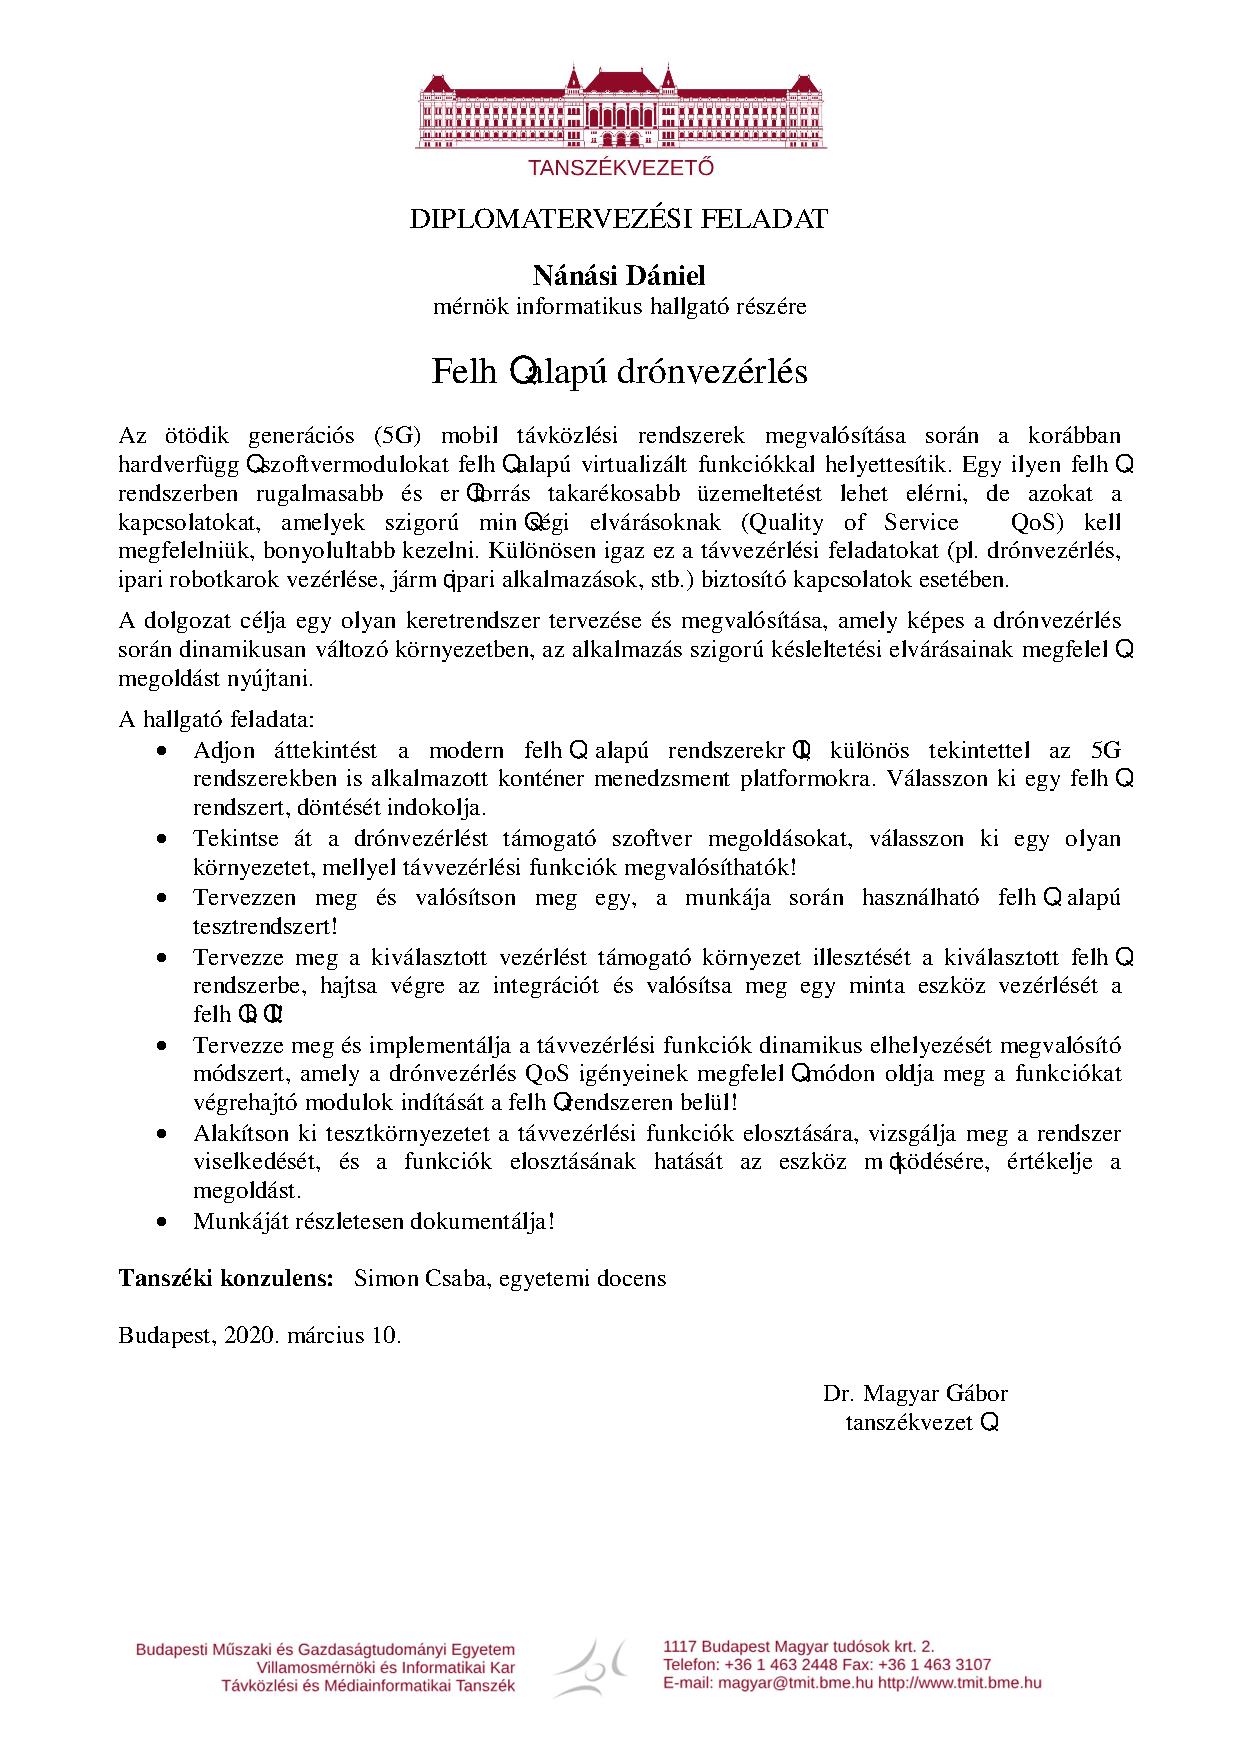
\includepdf[pages=-,pagecommand={},width=\linewidth]{include/project.pdf}

\selectthesislanguage

%~~~~~~~~~~~~~~~~~~~~~~~~~~~~~~~~~~~~~~~~~~~~~~~~~~~~~~~~~~~~~~~~~~~~~~~~~~~~~~~~~~~~~~
\hypersetup{pageanchor=false}
%--------------------------------------------------------------------------------------
%	The title page
%--------------------------------------------------------------------------------------
\begin{titlepage}
\begin{center}

\includegraphics[width=60mm,keepaspectratio]{figures/bme_logo.pdf}\\
\vspace{0.3cm}
\textbf{\bme}\\
\textmd{\vik}\\
\textmd{\viktanszek}\\[5cm]

\vspace{0.4cm}
{\huge \bfseries \vikcim}\\[0.8cm]
\vspace{0.5cm}
\textsc{\Large \vikdoktipus}\\[4cm]

{
	\renewcommand{\arraystretch}{0.85}
	\begin{tabular}{cc}
	 \makebox[7cm]{\emph{\keszitette}} & \makebox[7cm]{\emph{\konzulens}} \\ \noalign{\smallskip}
	 \makebox[7cm]{\szerzo} & \makebox[7cm]{\vikkonzulensA} \\
	  & \makebox[7cm]{\vikkonzulensB} \\
	  & \makebox[7cm]{\vikkonzulensC} \\
	\end{tabular}
}

\vfill
{\large 2020. December}
\end{center}
\end{titlepage}
\hypersetup{pageanchor=false}

		   % Szakdolgozat/Diplomaterv címlap

% Table of Contents
%~~~~~~~~~~~~~~~~~~~~~~~~~~~~~~~~~~~~~~~~~~~~~~~~~~~~~~~~~~~~~~~~~~~~~~~~~~~~~~~~~~~~~~
\tableofcontents\vfill

% Declaration and Abstract
%~~~~~~~~~~~~~~~~~~~~~~~~~~~~~~~~~~~~~~~~~~~~~~~~~~~~~~~~~~~~~~~~~~~~~~~~~~~~~~~~~~~~~~
%\selectlanguage{magyar}
\pagenumbering{gobble}
%--------------------------------------------------------------------------------------
% Nyilatkozat
%--------------------------------------------------------------------------------------
\begin{center}
\large
\textbf{HALLGATÓI NYILATKOZAT}\\
\end{center}

Alulírott \emph{\vikszerzoVezeteknev{} \vikszerzoKeresztnev}, szigorló hallgató kijelentem, hogy ezt a \vikmunkatipusat{} meg nem engedett segítség nélkül, saját magam készítettem, csak a megadott forrásokat (szakirodalom, eszközök stb.) használtam fel. Minden olyan részt, melyet szó szerint, vagy azonos értelemben, de átfogalmazva más forrásból átvettem, egyértelműen, a forrás megadásával megjelöltem.

Hozzájárulok, hogy a jelen munkám alapadatait (szerző(k), cím, angol és magyar nyelvű tartalmi kivonat, készítés éve, konzulens(ek) neve) a BME VIK nyilvánosan hozzáférhető elektronikus formában, a munka teljes szövegét pedig az egyetem belső hálózatán keresztül (vagy autentikált felhasználók számára) közzétegye. Kijelentem, hogy a benyújtott munka és annak elektronikus verziója megegyezik. Dékáni engedéllyel titkosított diplomatervek esetén a dolgozat szövege csak 3 év eltelte után válik hozzáférhetővé.

\begin{flushleft}
\vspace*{1cm}
Budapest, \today
\end{flushleft}

\begin{flushright}
 \vspace*{1cm}
 \makebox[7cm]{\rule{6cm}{.4pt}}\\
 \makebox[7cm]{\emph{\vikszerzoVezeteknev{} \vikszerzoKeresztnev}}\\
 \makebox[7cm]{hallgató}
\end{flushright}
\thispagestyle{empty}

\vfill
\clearpage
\thispagestyle{empty} % an empty page

\selectthesislanguage

%%\pagenumbering{roman}
%\setcounter{page}{1}

\selecthungarian

%----------------------------------------------------------------------------
% Abstract in Hungarian
%----------------------------------------------------------------------------
\chapter*{Kivonat}\addcontentsline{toc}{chapter}{Kivonat}

A diplomaterv a mai felhőrendszerekről és azokban robot irányítási megoldásaiban mélyed el.
Megmutatja a mai rendszerek felhőrendszerek szolgáltatás alapú technológiáit és bevezeti az olvasót a konténeralapú szolgáltatásmenedzsmentbe. Leírást ad a felhasználói igényekről és a felhőrendszereknek a jövőbeli fejlesztési lehetőségeiről. Áttekintést ad a közösségi fejlesztések által nyújtott nagy méretű erőforrás menedzsment megoldásoknak a mikéntjére, azok hibájára és bemutatja tesztelésüket. A dolgozat ismerteti és feldolgozza a mai robotirányítási megoldásokat, kifejezett prioritást tekintve a drón irányításnak, azoknak ipari felhasználásáról és megvalósíthatóságáról. Betekintést ad miként valósítható meg egy 5G kommunikációra alapuló robotirányításra tervezett felhőrendszer. Megmutat egy nagyobb számú robotot központi konténer alapú vezérlő és jelfeldolgozó rendszer megvalósítást. Továbbá kifejti ezeknek a tervezési és implementációs lépéseit és a távvezérlési funkciók dinamikus elhelyezését megvalósító módszert. Szimulációt mutat nagyszámú robotvezérlés és annak kamerajelének feldolgozására a kialakított rendszerben. Ennek tükrében összeveti a drónvezérlés QoS (Quality of Service) igényeinek feltételeit és a megvalósított rendszer funkcióinak ezen feltételrendszerre szabott tervezési megoldást ad a felhő rendszeren belül!
Összefoglalja az elvégzett munkát, a szimuláció eredményeit és a QoS feltételrendszert a kialakított tesztrendszerben.


\vfill
\selectenglish


%----------------------------------------------------------------------------
% Abstract in English
%----------------------------------------------------------------------------
\chapter*{Abstract}\addcontentsline{toc}{chapter}{Abstract}

The thesis delves into today’s cloud systems and the control solutions of individual robots.
It demonstrates today’s systems with cloud-based service technologies and introduces readers to container-based service management. Provides a description of user needs and cloud systems. Overview and a community development of large-scale resource management solutions is a way of failing and presenting their testing. The thesis describes and processes robot control solutions with explicit priority for drone guidelines, industrial use, and applicability. Provides insight into how to implement a cloud system designed for robotic control based on a 5G communication system. It focuses for larger number of robots in the operation of a central container-based control and signal processing system. In addition, it shows the design and implementation steps as well as the dynamic placement of remote control functions in the system design methodology. It analyses results of simulations in a system created to process a large number of robot controls and their camera signals. In order to improve quality, in order to facilitate the use of QoS (Quality of Service) and to facilitate the operation of the established system, the conditionalities usually becomes available.
Summarize the work, simulation, development and QoS conditions of the test system.

\vfill
\selectthesislanguage

\newcounter{romanPage}
\setcounter{romanPage}{\value{page}}
\stepcounter{romanPage}

% The main part of the thesis
%~~~~~~~~~~~~~~~~~~~~~~~~~~~~~~~~~~~~~~~~~~~~~~~~~~~~~~~~~~~~~~~~~~~~~~~~~~~~~~~~~~~~~~
\pagenumbering{arabic}
\chapter{Bevezetés}

Napjainkban a kisméretű repülő eszközöket, népszerű nevükön drónokat, sok feladatra használják. Jellemzően rádiós távvezérléssel, humán pilóta vezeti. Ugyanakkor elterjedőben van az automatizált feladatvezérlés is, de jelenleg főleg előre betáplált GPS koordináták sorozataként specikált útvonalat követnek. A mesterséges intelligencia technológia fejlődésével nagy reményt fűznek a feladatok programozott, adaptív logika alapú meghatározásával. Ebben az esetben a robotok vezérlését is meg kell oldani, a vezérlési logika által meghatározott koordináták alapján egy vezérlési központból küldik a parancsot a drónra. Mivel a vezérlési logika számításigényes, ezért ezt számítógép (adat) központokban futtatják és a vezérlési központ is a logika mellé van telepítve, valamint az adatközponotok tipikusan felhő rendszerként vannak megvalósítva. A munkám során egy ilyen felhőrendszerbe telepített vezérlési központ megvalósítási kérdéseivel foglalkoztam.

\section{Előzmények}

A dolgozatom témája felhő alapú drónvezérlés, amely több ágazatot, tématerületet ötvöz. Ugyanis a felhőtechnológiák, a robotvezérlés és az irányítástechnika spektrumot is lefedi a feladat, azonban én a felhőtechnológiák felől közelítem meg. A felhőalkalmazások ipara is egy ilyen terület, ahol bizonyos szolgáltatásokat minél szélesebb körben szeretnénk értékesíteni igény szerint, azonban valamilyen központi vezérlés működteti automatikusan az erőforráskiosztást, hozzáférést. A műhelyben végzett feladataim között felmerült a Kubernetes elosztott konténerkezelő rendszer, a Kubless serverless architektúra, felhő alapú beszédfelismerő rendszerek és az OpenStack virtuális gép menedzselő rendszer, amihez egy archiválási megoldást fejlesztettem szakdolgozatként. A felhő alapú drónirányítás téma a diplomatervem kezdetén került szóba, előtte nem foglalkoztam mélyebben robotirányítással és vezérléssel, így remélhetőleg ezekből a területekből is nagy tapasztalatot fogok szerezni a feladat befejeztén.

\section{A feladat célja}

\subsection{Feltételrendszer}
A feladat sokféleképpen általánosítható, hiszen egy felhőrendszerből igen sokféle ipari folyamatot lehet irányítani, csupán a megvalósítást kell kivitelezni. Egy drón irányítása sem különbözik, lehetne a cél robotkar vezérlése, gyártósor ütemezése, automatikus kötöttpályás közlekedési eszköz irányítása vagy akár önvezető autók feletti vezérlés.
 Azonban a témámban nem egy drón irányítását, hanem több, akár tíz-húszat is elérheti az a teszteset amire szeretnék megoldást adni. Egy ilyen rendszert irányító felhő architektrúban rugalmasabb és erőforrás takarékosabb üzemeltetést lehet elérni. A számításkapacitás optimalizáció nem minden amit ebben a helyzetben az ipar megkíván, hanem azokat a kommunikációs kapcsolatokat, amelyek szigorú minőségi elvárásoknak (Quality -of Service – QoS) kell megfelelniük, ezért bonyolultabb kezelni. A feladat feltérképezni a modern felhőrendszereket, amelyekkel meg lehet valósítani efféle iparban is használható vezérlési technikát QoS feltételek mellett. Tehát a projektnek három kritikus tervezési mérföldköve van. Ezeknek kapcsolata látszik a \ref{fig:merfold}. ábrán.
\begin{figure}
	\centering
	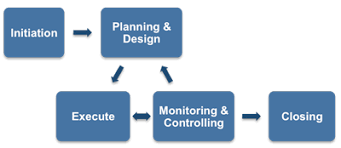
\includegraphics[width=10cm]{figures/plan_excecute_monitor.png}
	\caption{Kritikus mérföldkövek folyamata \cite{ProjecPlan}}
	\label{fig:merfold}
\end{figure}
\begin{enumerate}
	\item Kiválasztani a megfelelő felhőrendszert, amiben megvalósítható $R\in [1, 100]$ drón, vagy általánosan, valamilyen vezérelhető eszköz (robot) irányítása.
	\item Áttekinteni drónvezérlést támogató szoftver megoldásokat, kiválasztani egy olyan környezetet, mellyel távvezérlési funkciók megvalósíthatók. Megtervezni ebben a felhőrendszerben több drón irányítását és jelfeldolgozását, automatikusan és biztosítva, hogy hiba esetén visszaálljon a működő állapot.
	\item A meglévő rendszer analizálása, optimalizálása és egy QoS feltétel felállítása.
\end{enumerate}

\subsection{Vezérlési feladatok erőforrásigénye}
\noindent
Dolgozatom célja nem csak a drónirányítórendszer megvalósítása, hanem annak kapacitásának megbecslése is, akár  több tíz drón irányítására. Ezt a feltételt valamilyen $f_{QoS}(R,C)\in N^2$ függvény fogja megadni, melynek paraméterei $R$ a robotok száma és $C$ a számítási erőforrás. Ha számításról beszélünk, akkor a felhőszolgáltatások iparában kiválasztunk egy valamilyen optimális $c=$RAM[GB]/VCPU arányt mely az alkalmazásunkhoz megfelelő és annak $n\in N^+$, $C=c\cdot n$ egész számú többszöröse lesz a számítási kapacitás amire méretezünk. Vagyis valamilyen 2 dimenziós tervezési teret adunk meg a kívánt szolgáltatási minőség eléréséhez. Az ilyen jellegű feladatokban a szolgáltatás minősége általában a válaszidőt szokta jelenteni $n \cdot 10$-es nagyságrendben. Természetesen ez nem egy túl pontos modell, de egy mérnöki kapacitástervezés számára kellő kiindulási alapot adhat méretezni a felhőrendszert, esetleg skálázhatósági lehetőségeket is figyelembe véve.
Ezen kívül mivel nagyszámú eszközről beszélünk nem tekinthetünk el a közegátviteli technológiáról. Azt sejthetjük, hogy a mai elterjedt távközlő rendszerek nem alkalmasak akár száz fölötti felhasználóval, mondjuk robottal folyamatos kommunikációt tartani megfelelő QoS-el. Ezért megnézem, hogy a mai modern felhőrendszerekkel és az 5G között milyen kapcsolatot lehet alakítani és mik a feltételek egy ilyen rendszerben való üzemeltetéshez. \\

\subsection{Elvárások a rendszerrel szemben}
\noindent
A feladat megvalósított terméke pedig egy valamilyen automatizált felhőrendszerbe ültetett drónirányító központ melynek segítségével $N$ darab virtuális vagy fizikai drónt tudunk üzemeltetni, az előző bekezdésben taglalt QoS feltételek mellett. Fontos, hogy a drónirányító központban minden kommunikációt tudjunk kontrollálni és biztonságos állapotba helyezni a drónokat, hogyha tudjuk, hogy valamely biztosítandó alapfeltételnek nem tesz eleget pillanatnyilag a rendszerünk. Tehát amit meg kell valósítani a mérések mellett az nem más, mint egy felhőrendszerbe integrált szoftver, amely biztosítja 
\begin{itemize}
	\item előre definiált $N$ darab drón irányítását a felhasználónak, a felhőből kivezetett interfészen,
	\item minden drónra vonatkozó kamerakép és irányítási parancsok átviteli sebessége, előre definiált konstans alapján,
	\item a drón és felhő közötti kapcsolatot egy előre definiált minimum sávszélesség alapján,
	\item amennyiben az előző feltételeknek nem tesz eleget a rendszer, a biztonságos leállítását az összes drónnak.
\end{itemize}

\subsection{Sávszélesség}
\noindent
Ezen feltételek mellett felírhatunk pár egyszerű összefüggést egy vázlatos modellre, aminek blokkdiagramja a \ref{fig:dronecommunicationtocloud}. ábrán látható. Tudjuk, hogy lesz egy valamilyen még ki nem választott felhőrendszer, amely biztosan több node-ból fog állni, tehát több fizikai vagy virtuális gép fogja szolgáltatni a felhőrendszer platformját. A node-ok között feltételezzük, hogy nincs sávszélességi korlát. A felhőrendszer szolgáltat valamilyen interface-t amint elérhető az integrált szolgáltatás a drónok számára. Ezen modellen következik, hogy a hálózati interface és a tényleges integrált applikáció közötti sávszélességnek nagyobbnak kell lennie, mint a drón felé a sávszélesség összessége:
\begin{equation}
BWc \geq \sum_{i=1}^{n}{BWd_i}
\end{equation}

A drónok sávszélességére felírhatjuk azt a feltételt, amely kimondja, hogy bármely drón sávszélességének nagyobbnak kell lennie, mint a videófolyamhoz rendelt minimális sávszélességnek és az irányításhoz megszabott minimális irányíthatósági sávszélességnek.
\begin{equation}
\forall d \in D: BW_d \geq BWV_{min} + BWC_{min}
\end{equation}
Ahol $BWV_{min}$ a videó minimális sávszélessége, $BMC_{min}$ a kontrollerhez rendelt minimális sávszélesség, $BW_d$ az adott drón és a felhő közötti sávszélesség, $D$ pedig a drónok halmaza.

\begin{figure}
	\centering
	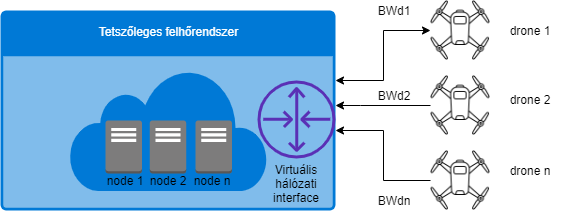
\includegraphics[width=\linewidth]{figures/drone_communication_to_cloud.png}
	\caption{A drónok és felhő kapcsolatának vázlatos modellje}
	\label{fig:dronecommunicationtocloud}
\end{figure}

\section{Feladat indokoltsága}
\subsection{Gyártóipar}
A nagyszámú eszközök irányítása számtalan szektorban elterjedt és alkalmazható. Akár beszélve a gyártó szektorról, ahol nagyon sok folyamatot robotok látnak el és legyen az bármilyen robot, az valószínűleg irányítható felhőből. Persze sokszor a gyártók egy drágább, de kapacitásban túlbiztosított lokális rendszerről irányítják a gyártórobotjaikat, mivel a felhős megoldások még annyira nem elterjedtek ebben a célfelhasználásban. Azonban egy ilyen megoldással rengeteg erőforrás megtakarítható.
A \ref{fig:industry40}. ábrán láthatóak az Ipar 4.0 főbb komponensei és könnyen meggyőződhetünk róla, hogy egy mai innovatív ipari környezetben inkább a felhő alapú megoldásokat választják a skálázhatóság és a biztonságuk miatt. Ebben az esetben felhőről általában számítási kapacitásról beszélünk, azonban később kitérünk a szolgáltatások kategóriáira.
\begin{figure}
	\centering
	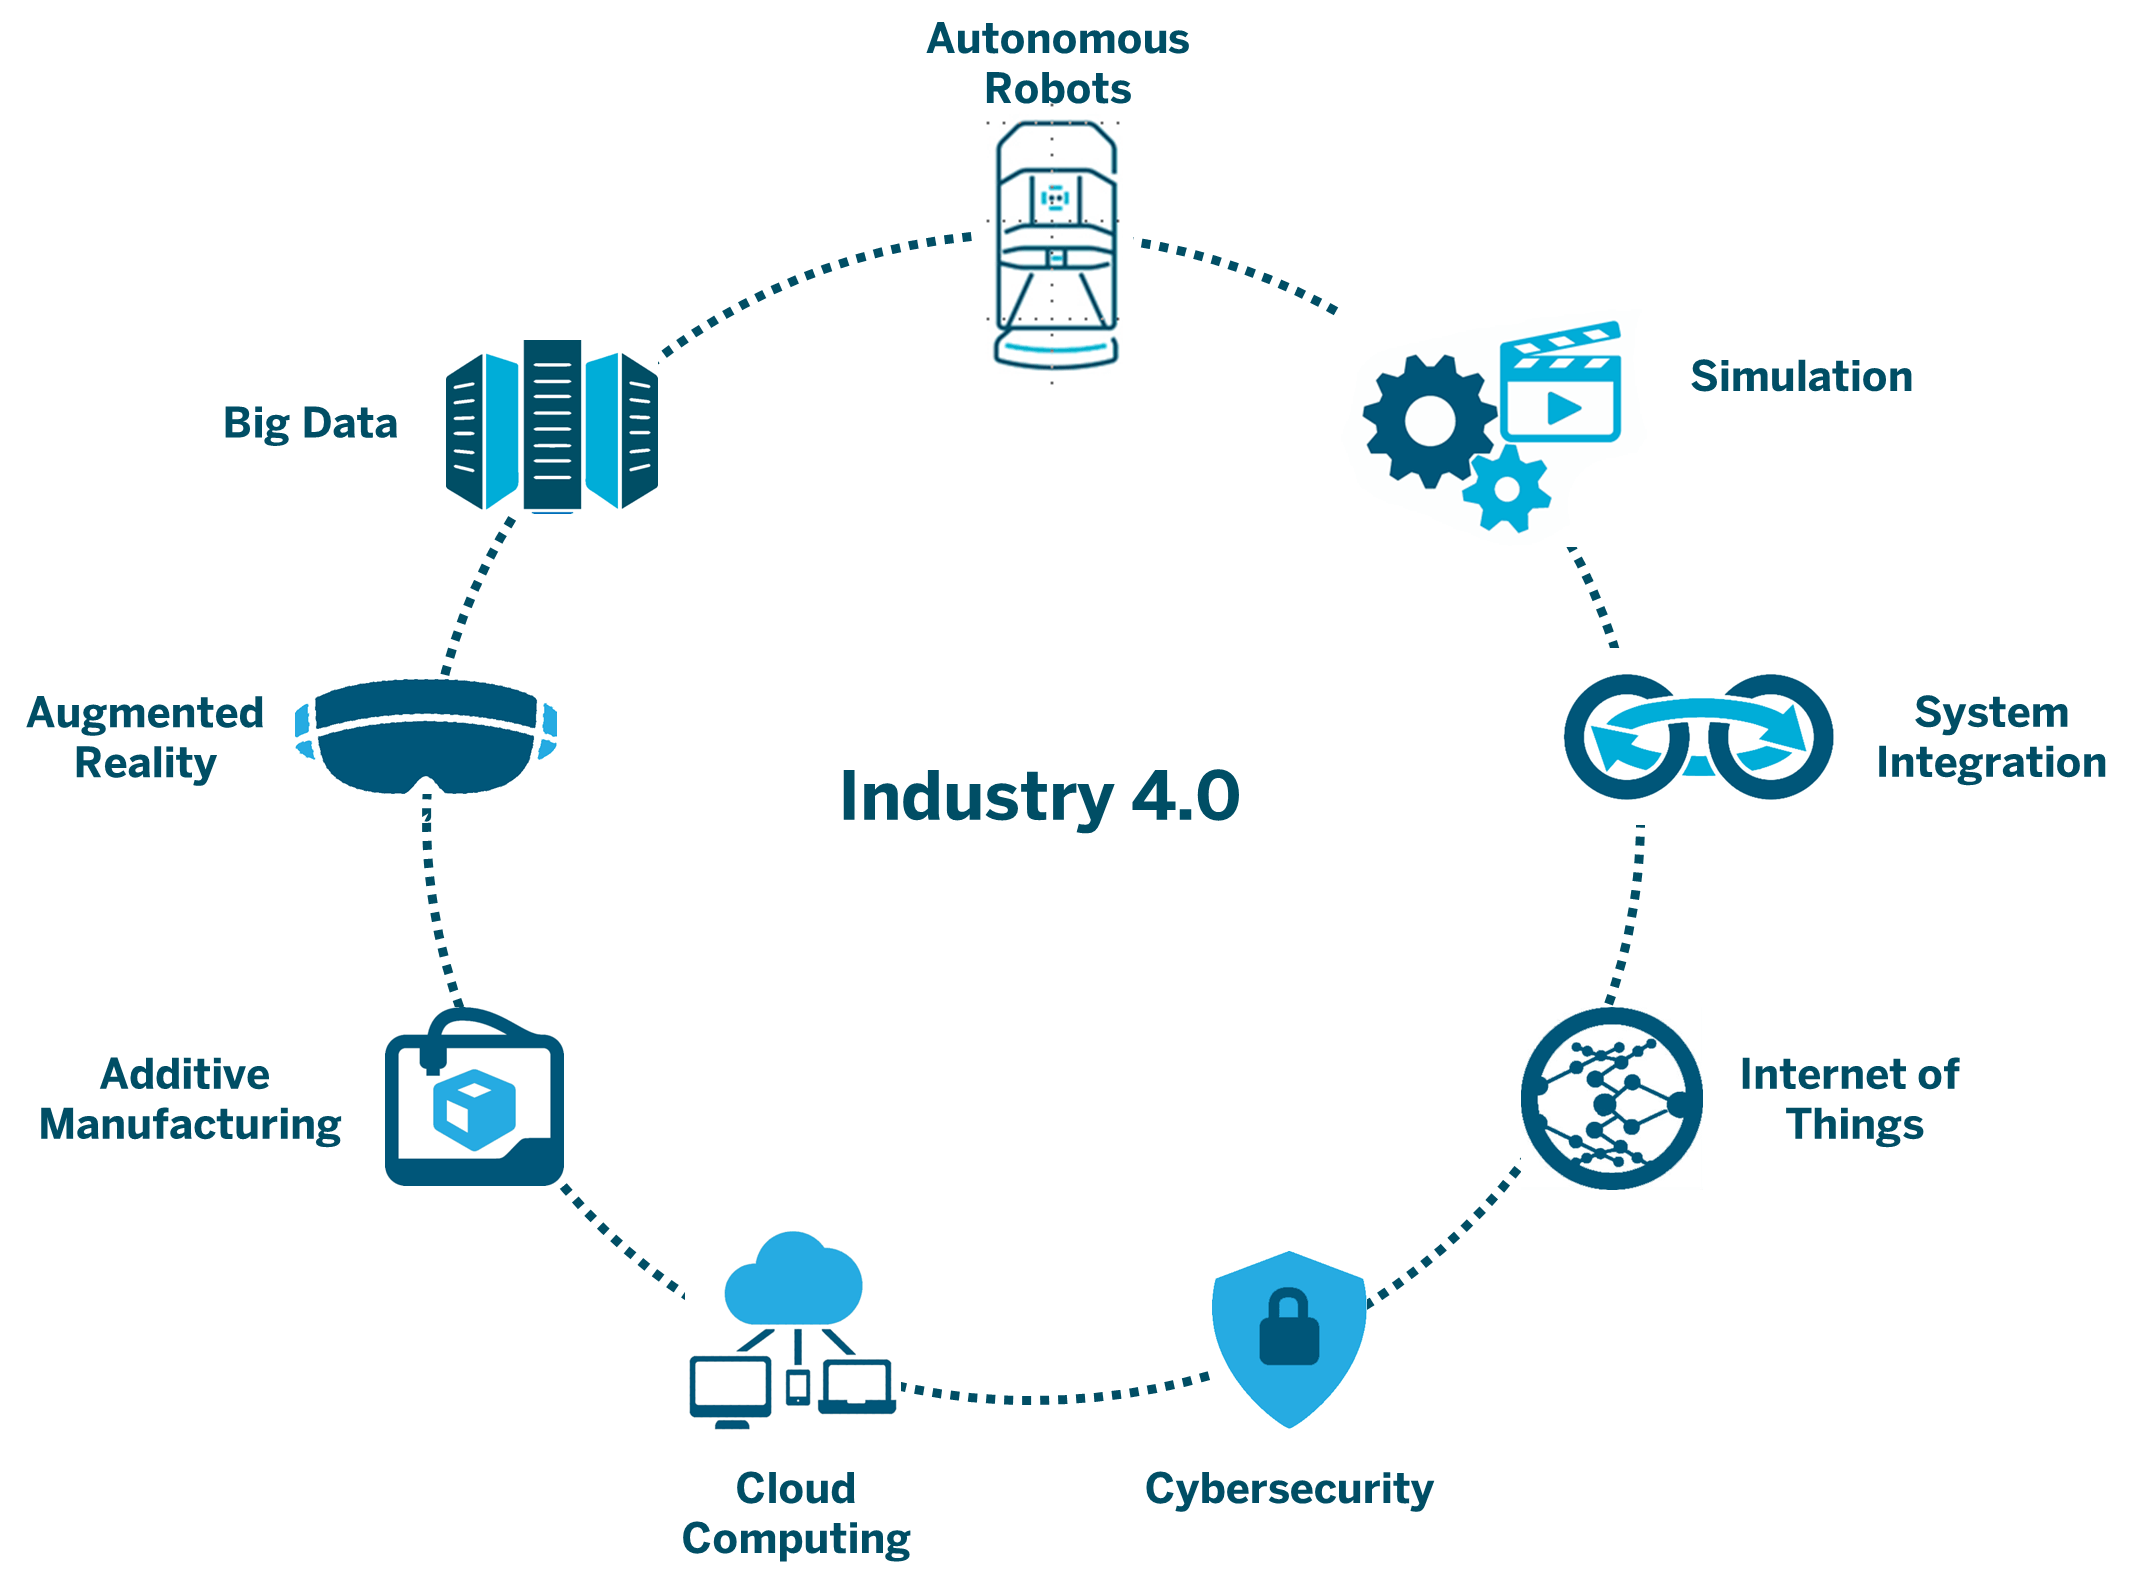
\includegraphics[width=\linewidth]{figures/industry40.png}
	\caption{Ipar 4.0 komponensei \cite{industry40}}
	\label{fig:industry40}
\end{figure}

\subsection{Szállítás}
Nem csak a gyártóiparban lehet elképzelni sok robot irányítását, hanem például szállítás és utazás terén is. A Műegyetemhez legközelebbi metróvonal már évek óta önvezérlőként működik, ugyan egyelőre a hossza befejezetlensége miatt csak tíz körüli metrószerelvény működik egyszerre, azonban ez is egy olyan példája a robotirányításnak, amit minden nap észlelhetünk. Az Amazon házhozszállító cég, amelynek egyébként az AWS (Amazon Web Services) leányvállalata a világ egyik legnagyobb felhőszolgáltatója, már tesztel drónokat, amelyek betöltik a csomagházhozszállítás szerepet. A levegőben való csomagszállítás egyik problémája a \ref{fig:drone-delivery}. ábrán látható.
\begin{figure}
	\centering
	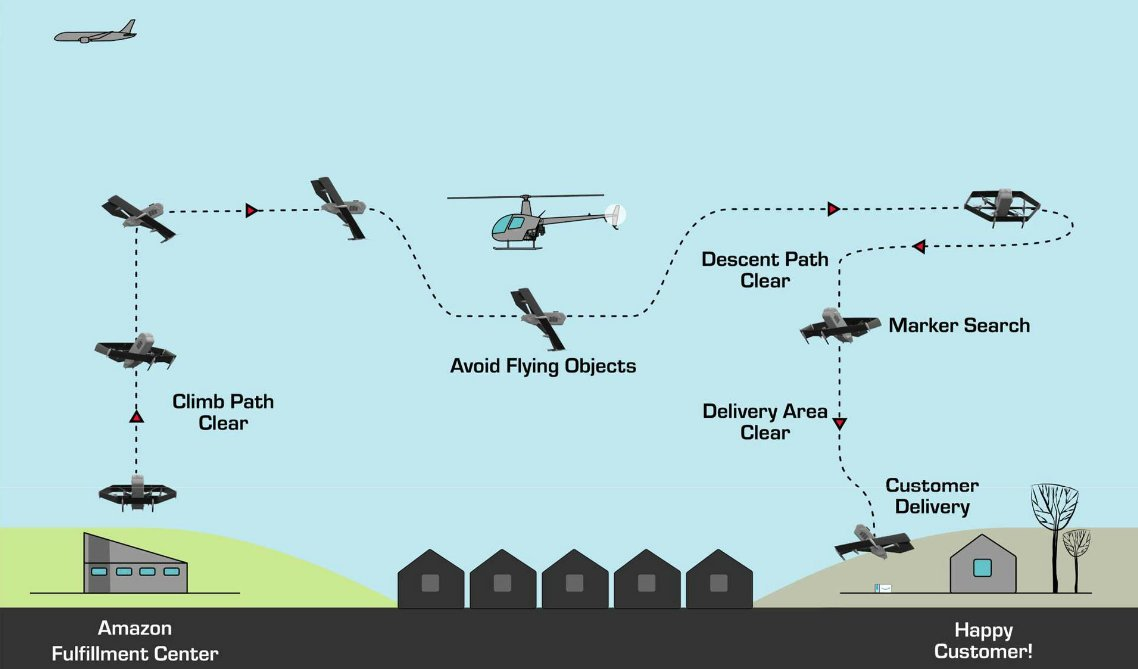
\includegraphics[width=\linewidth]{figures/aws-drone-delivery.jpg}
	\caption{Amazon házhozszállítás problémája drónnal \cite{drone-delivery}}
	\label{fig:drone-delivery}
\end{figure}
\subsection{Mezőgazdaság}
Az agrárvilágban is el lehet képzelni sok robotot kezdve a vetéstől az aratásig, azonban a drónoknak kifejezett szerepe akad a jövőben ebben az iparágban. Használnak ma már automatizált drónokat permetezésre, időszakos állomány megfigyelésre vagy akár kombájn útjának a felderítésére is. Ahogyan a gyártósoroknál, itt is optimalizálhatunk több robot irányítás esetén felhőrendszerrel. A dolgozatban arra keresünk megoldást, hogy ezt milyen eszközrendszerrel érdemes tervezni.
\subsection{Szórakoztatóipar}
Idáig kiderült, hogy rengeteg iparágban alkalmazhatóak a tömegesen irányított robotok, amiket kreativitással könnyű bővíteni. Azonban a szórakoztatóiparban is megjelentek már a tömegesen irányított drónok. Egy jellegzetes példája ennek amerika legnagyobb sporteseménye a Super Bowl 2017-es döntője, ahol 300 drónt használtak fel az égboltra való fényfestéshez a szünetben lévő koncerthez. Ez az esemény egy pillanatfelvétele a \ref{fig:super-bowl}. ábrán látható és az esemény technikai előkészületeiről a \cite{concert} cikkben lehet olvasni.
\begin{figure}
	\centering
	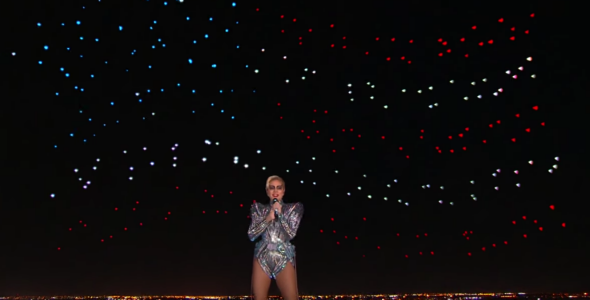
\includegraphics[width=12cm]{figures/super_bowl.png}
	\caption{Lady Gaga 300 drónnal a háttérben a 2017-es Super Bowl döntőjének félideje alatti koncerten \cite{super-bowl-pic}}
	\label{fig:super-bowl}
\end{figure}
Persze ebben a példában egy pár perces feladatról beszélünk az irányított robotok számára, a felhős megoldással pedig egy hosszútávú optimalizációt szeretnénk megadni.

\section{Használt kifejezések}
A hálózati-, virtualizációs- és robotiparban rengeteg rövidítés, mozaikszó és kifejezés létezik, amit főként csak azok ismernek, akik
jelentősebben mélyültek el ezen iparág területén. Két csoportra bontom a diplomatervemhez használt kifejezéseket:
\begin{enumerate}
	\item Azon szakmai kifejezések, amik elterjedtek a mérnöki szakmákban, melyet egy mérnök nem infokommunikációs szakosodás mellett is nagy valószínűséggel ismer és nem kell ismertetnem a tanulmányban. Pár példa a kategóriában, amikre külön nem térek ki, nem oldom fel a szövegben, ilyenek az IPv4, NAT, hálózati réteg, HTTP, CPU, for ciklus.
	\item Azokat a kifejezéseket amik pedig a témához, szakterülethez kapcsolódnak, például a kifejezetten hálózati kommunikáció, virtualizáció, robot, irányítás iparágakba tartozó kifejezések, amiket nem általános mérnöki ismeretek, azokat a szövegben az első használatnál kifejtem, továbbá itt összegyűjtöm.
\end{enumerate}
A tanulmányban használt speciális kifejezések:
\begin{itemize}
	\item QoS (Quality of Service) - A szolgáltatás minőségének a biztosítása
	\item Virtuális gép (Virtual Machine, VM) - Virtualizált önálló teljes értékű operációs rendszer gazdagépen (host-on)
	\item KVM (Kernel-based Virtual Machine) - Kernelhez elosztott időben hozzáférő virtuális gép
	\item Host OS - Hosted virtualizáció esetén a gazdaoperációs rendszer
	\item Guest OS - Hosted virtualizált operációs rendszer a host OS fölött
	\item Hypervisor - A hardveren való virtualizációt megvalósító szoftver
	\item Node - A felhőrendszer egy fizikai eszköze
	\item Cluster/Klaszter - A felhőrendszerbe csatolt fizikai eszközök kapcsolata
	\item Volume - Szolgáltatás/VM háttértára
	\item Vertikális skálázás - Node hozzáadása a cluster-hez
	\item Horizontális skálzás - Node fejlesztés
	\item GCS (Ground Control Station) - Földi irányítóállomás
	\item Földi - Olyan alkalmazás ami nem felhőben fut
	\item Konténer Registry - Konténereket tároló és menedzselő rendszer
\end{itemize}
\chapter{Felhőrendszer kiválasztása}
\label{cha:cloud}
A számítás alapú felhőrendszereknek két alapja van, a teljes virtualizált önálló operációsrendszer (VM, mint Virtual Machine) vagy pedig a konténerizált, önálló lebutított virtualizált operációs rendszer szolgáltatás szinten.
Egy platform virtualizációja olyan virtuális gép létrehozását jelenti, amely egy valós operációs rendszerű számítógépként működik. A virtuális gépeken végrehajtott szoftverek elkülönülnek az alapul szolgáló hardverforrásoktól.

\section{Virtualizációs alapok}
A KVM (Kernel-based Virtual Machine, azaz kernel alapú virtuális gép), egy teljes
virtualizációs megoldás amely képes kihasználni az újabb processzorokban rejlő hardveres
virtualizáció képességet. Magában foglal egy betölthető kernel modult, alkalmas egy adott operációs rendszeren virtualizált környezetben egy másik operációs rendszert futtatni. Azaz miközben a gazda operációs rendszer fut a számítógépen addig képesek vagyunk egy másik vendégrendszert indítani virtuális környezetben. Ettől ez a megoldás sokkal gyorsabb.



\subsection{Hypervisor}
Szoftverben megvalósított menedzser a virtuális gépek számára. A gazdahardveren fut,
lehetővé teszi a vendég gépek (guest OS) futtatását, memória kezelését és processzor ütemezését különböző
algoritmusokkal. Két főbb típust különböztetünk meg. 
\paragraphl{Bare matel}
Az első típusú hypervisorok közvetlenül a hardverre vannak telepítve.
Tartalmazniuk kell saját operációs rendszerüket a rendszerindításhoz, a hardver futtatásához és a
hálózathoz való csatlakozáshoz. Ilyen hypervisor pl. a Microsoft Hyper-V. 
\paragraphl{Hosted}
A hosztolt hypervisorok olyan operációs rendszereken futnak, amely közvetlenül a hardverre van telepítve. Ebben az esetben szükség van egy gazda operációs rendszerre (host OS).
\subsection{Konténer}
A konténerizáció egy olyan megoldás, ahol a szolgáltatásokat külön-külön letisztult operációs rendszerre telepítjük és csak azokat a szoftvereket ami az adott szolgáltatáshoz szükséges. A konténerizáció elszeparálása a Linux kernel namespace technológiáján alapul. Működésük alapján hasonlítanak a VM-ekre, úgy is lehet mondani, hogy egy olyan VM optimalizált megoldása, amin egy applikáció fut. Egy rendes operációs rendszeren futó számítógépes program képes megtekinteni az adott rendszer összes erőforrását (csatlakoztatott eszközök, fájlok és mappák, hálózati megosztások, CPU-teljesítmény, számszerűsíthető hardver-
képességek). A konténeren belül futó programok azonban csak a konténer tartalmát és eszközeit látják el.
\subsection{Docker}
A Docker a legelterjedtebb konténerizáció megoldás, 2013-ban kiadott technológia Windows és Linux operációs rendszerekhez. A Docker elsősorban Linuxra készült, ahol a Linux kernel erőforrás-elkülönítési jellemzőit (cgroup-okat), a névtereket és a fájlrendszert használja, . Ezek lehetővé teszik a független konténerek egyetlen Linux példányán működését, elkerülve bármilyen összeférhetetlenséget.
\paragraphl{Hálózata}
A docker konténereknek 3 féle hálózati interface-ük lehet,
\begin{itemize}
	\item Host - kívülről elérhető
	\item Bridge - a docker konténerek elérik egymást
	\item None - nincs hálózatra kötve
\end{itemize}
\paragraphl{Port forward}
Docker konténerek létrehozásánál megadhatjuk a port átirányítást, így azonos alkalmazások sem akadnak össze.
\begin{minipage}{\linewidth}
\begin{lstlisting}[caption={Példa két WordPress szolgáltatás párhuzamos indítására a 80 és 81-es portokon}]
$ docker run --name wp1 wordpress
$ docker run --name wp2 -p 80:81 wordpress
\end{lstlisting}
\end{minipage}
\paragraphl{Volume csatolás}
Alapvetően nehézkes hozzáférni a konténer belső tárhelyéhez, azonban gazda OS alatt tudunk csatolni a szolgáltatáshoz tartozó könyvtárat a host OS fájlrendszeréhez.
\begin{lstlisting}[caption={Példa volume csatolásához}]
$ docker run -v /usr/local/mywordpress:/wordpress wordpress
\end{lstlisting}
\paragraphl{Példa docker konténer robotoperációsrendszerhez}
A robotoperációs rendszerekről később lesz szó, azonban megadok egy példát ilusztrálva, hogyan alakítható egyszerá szolgáltatás docker konténerré, csupán egy Dockerfile nevű fájlra van szükség az applikáció főkönyvtárában (\ref{lst:dockerexample}. számú kódrészlet).

\begin{minipage}{\linewidth}
\begin{lstlisting}[caption={Példa alap robotoperációsrendszer konténerizációjához}, label={lst:dockerexample}]
FROM ros:melodic-ros-base

RUN apt-get update && apt-get install locales -y
RUN locale-gen en_US.UTF-8
ENV LANG en_US.UTF-8

COPY . /catkin_ws/src/
WORKDIR /catkin_ws
RUN /bin/bash -c '. /opt/ros/kinetic/setup.bash; catkin_make'
RUN /bin/bash -c '. /opt/ros/kinetic/setup.bash; source devel/setup.bash'

CMD ["roslaunch", "bebop_gazebo bebop_moving_helipad.launch"]
\end{lstlisting}
\end{minipage}
A \emph{FROM} parancsal a szülő konténert adom meg, amit DockerHub-ról automatikusan letölt, a \emph{RUN} parancsokkal környezeti programokat telepítek, \emph{COPY} az applikációhoz tartozó fájlokat másolja a konténerbe, \emph{ENV} paranccsal környezeti változót állítok, \emph{WORKDIR} parancs a munkakönyvtár beállítása és a \emph{CMD} utasítás a konténerizáltan futtatandó applikáció megadása.

\section{Docker Compose}
A Compose egy multi-konténer Docker eszköz különböző alkalmazások együttes definiálásához és működéséhez. A Compose használatával YAML fájlban definiálni lehet különböző konténereket más-más paraméterekkel szolgáltatásainak konfigurálására. Ezután egyetlen paranccsal elindíthatóak a docker konténerek, az összes együtt működő szolgáltatás a konfigurációból. \cite{compose} A feladathoz biztosan kell használni, mivel a drónirányítás több különböző funkcióból valósul meg, így a konténer definíciója szerint érdemes minden egyes applikációt elkülöníteni és Compose-al összekötni a működésüket.

\section{Docker Swarm}
A Docker Swarm olyan fizikai vagy virtuális gépek (node-ok) csoportja, amelyek futtatják a Docker alkalmazást, és amelyeket együttesen egy swarm-t alkotnak, hogy összekapcsolódjanak egy clusterként. Miután egy csoport node-ot összekapcsoltak, továbbra is futtható rajtuk a Docker vezérlőparancsok, ezeket most a worker node-ok hajtják végre. A klaszter tevékenységét egy swarm manager irányítja, és a klaszterhez csatlakozó gépeken osztja ki a feladatokat. A docker swarm manager és worker node-ból áll és alkalmazható a swarm-ra a docker compose is (\ref{fig:swarm}. ábra).
\begin{figure}
	\centering
	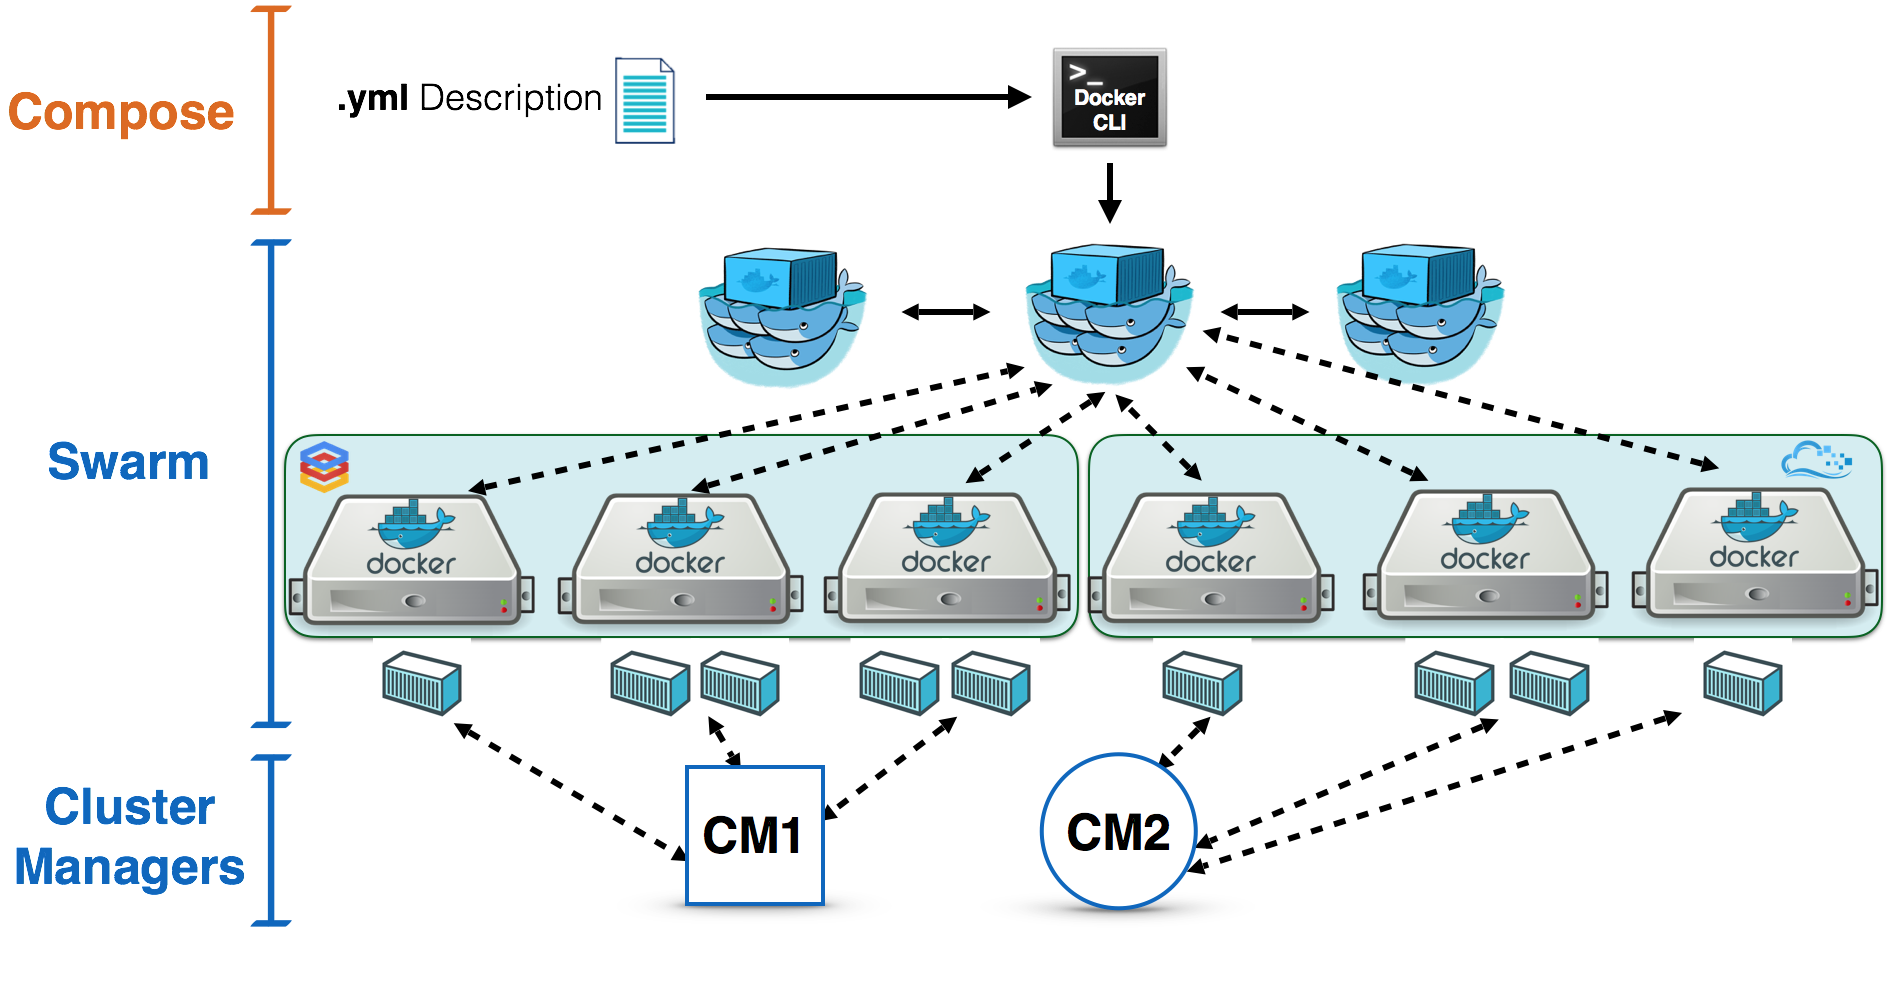
\includegraphics[width=\linewidth]{figures/swarm.png}
	\caption{Docker Swarm architektúra \cite{docker-swarm}}
	\label{fig:swarm}
\end{figure}

\section{Mesos}
A Mesos az Apache szoftvere, mely egy absztrakt környezetet hoz létre CPU, RAM és háttértárral, akár 10.000 node-ig. A Mesos egy nyílt forrású cluster kezelő szoftver. Alkalmazásokat kínál API-kat az erőforrás-kezelésre és az ütemezésre a cluster-en keresztül.  A Mesos rugalmasságot és az elhaló alkalmazások újraindítását biztosítja. Lehetővé teszi a framework-ök számára, hogy ütemezzék és végrehajtják a feladatokat API-n keresztül. A Mesos-architektúra egy master node-ból áll, amely az egyes node-okon futó worker-eket és a worker-eken futó framework-öket kezeli, melyeken a szolgáltatások futnak. Az összes alkalmazásdefiníció egy JSON-fájlban található, amelyet továbbítanak a Mesos / Marathon REST API-hoz.

\section{Kubernetes}
Egy docker rendszerben a definiált konténer egy példánya futtatható a \emph{docker run} utasítással. Kubernetest használva a kube control CLI-on keresztül akár ezer példánya is futtatható ugyanannak az alkalmazásnak.
\begin{lstlisting}[caption={Példa 100 alkalmazás indítására}]
$ kubectl run --replicas=100 wordpress
\end{lstlisting}
A futtatott alkalmazásokat egy másik parancsal felskálázhatjuk.
\begin{lstlisting}[caption={Példa alkalmazás skálázására}]
$ kubectl scale --replicas=200 wordpress
\end{lstlisting}
Tehát egy kihasználtsági emelkedő esetén egyszerűen lefoglalhatunk több erőforrást a felhasználás tekintetében.
A Kubernetes a Docker host programot használja az egyes node-okon alkalmazások futtatásához. Alapvetően konténerekret támogat, azonban nem csak a Docker-t, hanem pl. a Rocket-et és a Cryo-t is.
\subsection{Architektúra}
Egy Kubernetes cluster architektúrája fizikai vagy VM node-okból áll és minden node egy worker (\ref{fig:kubearch}. ábra). Egy node meghibásodása esetén a rajta futó service-t átveszi a többi node. A node-ok között van egy kitüntetett master node, amelyik tárolja a cluster információkat és végzi a manager service-ek processzeit.

\begin{figure}
	\centering
	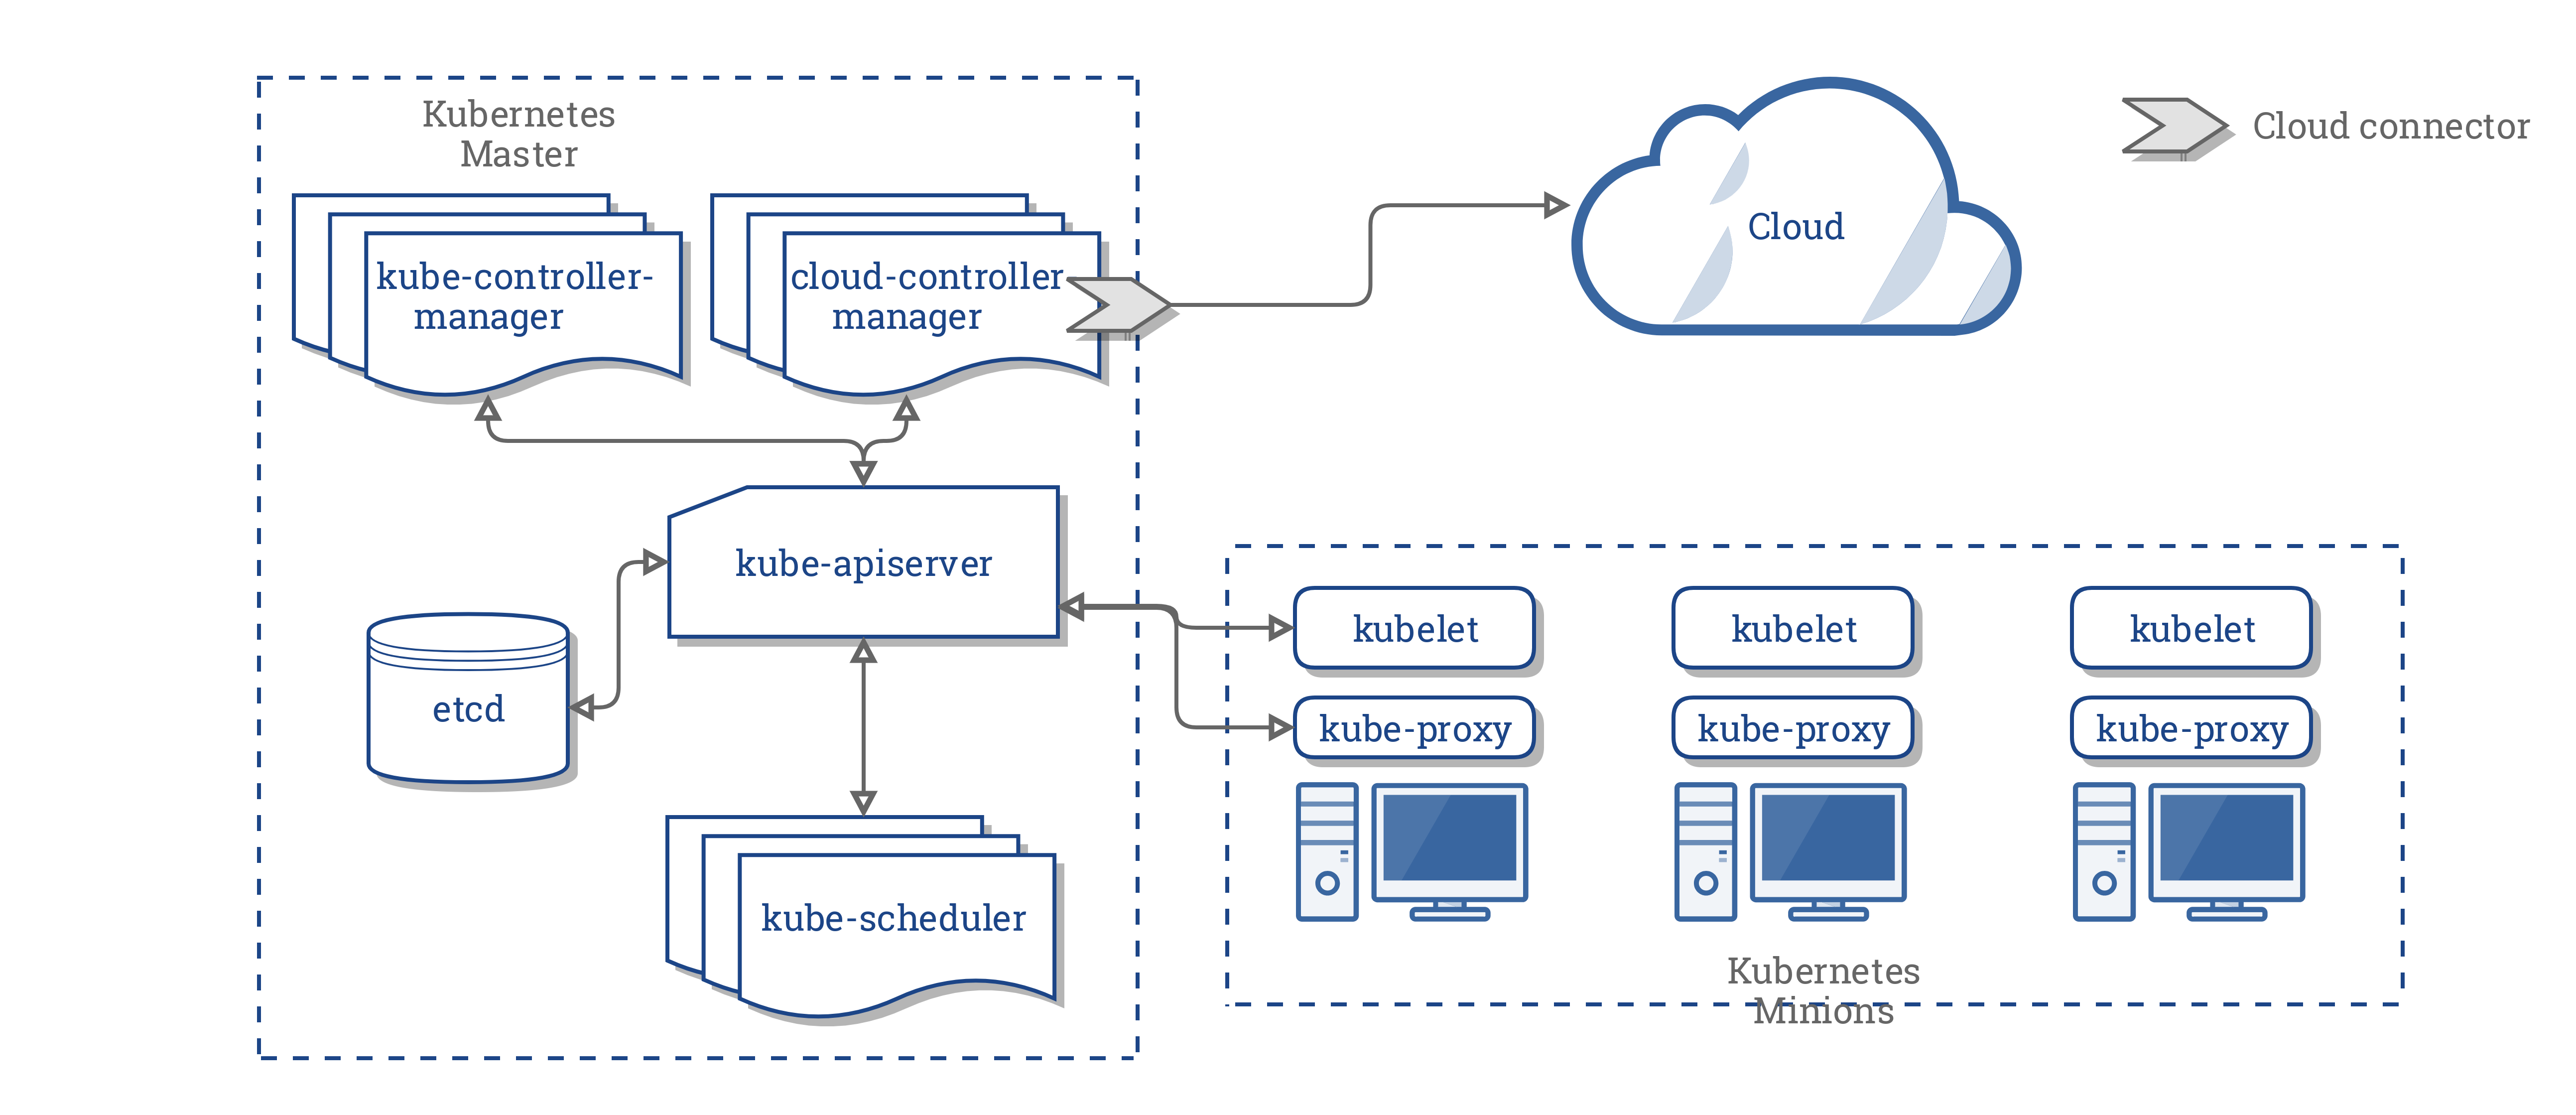
\includegraphics[width=\linewidth]{figures/kube_arch.png}
	\caption{Kubernetes architektúrája \cite{kube-arch}}
	\label{fig:kubearch}
\end{figure}

\subsection{Komponensek}
\paragraphl{API server}
A Kubernetes frontend-jét web UI-t és API-t szolgáltat. Ezzel kommunikál a felhasználó menedzser, CLI-t és a többi UI eszköz is. 
\paragraphl{etcd}
Elosztott kulcsérték tároló, a cluster menedzseléséhez szolgáló információknak.
\paragraphl{Scheduler}
Az elosztott működést valósítja meg a node-okon, minden új feladatot eloszt egy node-hoz.
\paragraphl{Controller}
Figyeli a végpontokat és beavatkozik ha valami tönkremegy.
\paragraphl{Container runtime}
A konténerek keretszoftvere, leggyakoribb esetben a Docker.
\paragraphl{Kubelet}
Ez a service minden node-on fut a cluster-en, a feladata, hogy a node-hoz kiszervezett konténerek fussanak az elvárt módon.
\paragraphl{Kube control}
CLI, amin keresztül az adminisztrátor tud szolgáltatásokat indítani és cluster menedzsment feladatokat ellátni.


\section{Keretrendszer meghatározása}
A nagyszámú robotvezérlés feladatkörében hasonlítom össze a három legelterjedtebb orkesztrációs megoldást.
\begin{center}
	\begin{table}
	\begin{tabular}{ |p{5cm}|p{3cm}|p{3cm}|p{3cm}|  }
		\hline
		\multicolumn{4}{|c|}{Konténer orkesztráció rendszerek} \\
		\hline
		&
		\begin{minipage}{.3\textwidth}
			
\includegraphics[width=3cm]{figures/docker_swarm.png}
		\end{minipage} 
		&
		\begin{minipage}{.3\textwidth}
			
\includegraphics[width=3cm]{figures/mesos.png}
		\end{minipage} 
		&
		\begin{minipage}{.3\textwidth}
			
\includegraphics[width=3cm]{figures/kubernetes.png}
		\end{minipage} 
		 \\
		\hline
		Konténerre optimalizált & \cmark & \xmark & \cmark \\
		Egyszerű telepítés & \cmark & \xmark & \xmark \\
		Szolgáltatás skálázhatóság & \xmark & \xmark & \cmark  \\
		Horizontális skálázhatóság & \cmark & \cmark & \cmark \\
		Vertikális skálázhatóság & \xmark & \cmark & \cmark \\
		Multi-konténer deploy & \cmark & \xmark & \cmark \\
		Minimum node & 1 & 3 masters + slaves & master + 2 slaves \\
		\hline
	\end{tabular}
	\caption{Konténer orkesztrációs rendszerek összehasonlítása}
	\end{table}
\end{center}
A vezérlési rendszerre legoptimálisabb választás a \textbf{Kubernetes}.
\paragraphl{Indoklás}
Egy QoS minőségbiztosított alkalmazás számár nagyon fontos a skálázhatóság és a perzisztencia. Ha kiesik egy node, akkor is fontos, hogy egy kis lassulással is, de stabil maradjon a szolgáltatás. Nagyon jól kezel multi-konténer alkalmazásokat, könnyű a szolgáltatás működése közben új konténereket indítani. A minőségbiztosítási feltételeket a Kubernetes biztosítja a legjobban.

\chapter{Drónvezérlés környezete}
\section{Robotirányítás}
Robotirányításhoz szükséges, hogy legyen egy mechanikai rendszer, ez a robot azon részrendszere, amely az akciót valósítja meg. Az akció során szükség lehet a robot mozgatására a környezetben,
ezt a helyváltoztató berendezés végzi. Motorok, különböző mechanikai tagok teszik lehetővé a helyváltoztatást. A szenzoros rendszer belső állapota maga a mechanikai rendszer állapota, míg a külső állapot a környezet állapotát jellemzi.
Sokféle külső környezeti állapot létezik. Ahhoz, hogy a különböző környezeti tényezőket, például hőmérséklet, fényerősség, mágnesesség, láthatóvá és érzékelhetővé tegyük a robotunk számára, fel kell szerelni a megfelelő szenzorokkal.
A dolgozat során egy Mantis Q drónt (\ref{fig:mantisq}. ábra) használunk robotként, a többit szimuláljuk.

\begin{figure}
	\centering
	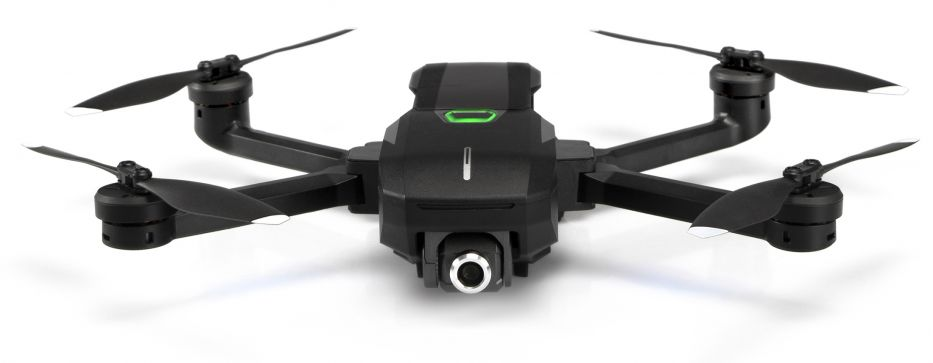
\includegraphics[width=\linewidth]{figures/mantisq.jpg}
	\caption{Yuneec Mantis Q \cite{mantisq}}
	\label{fig:mantisq}
\end{figure}

\section{Robot operációs rendszer - ROS}
Bármilyen robot rendelkezik különféle eszközökkel amivel érzékelik a világot és mozognak benne. A Robot operációs rendszer egy nyílt forráskódú könyvtárakat és eszközöket kínál a szoftverfejlesztés segítségére robotot, mint hardvert irányító alkalmazások létrehozásához. Hardver abszrakciót, driver-eket, könyvtárakat, megjelenítőket, üzenetek továbbítását, csomagkezelést és más szolgáltatást is nyújt. \cite{roswiki}
A ROS node-ok kommunikálni tudnak egymással, a szolgáltatások, hogy kérést küldjenek és választ kapjanak a node-ok között. A \emph{rosservice} szolgáltatással kapcsolódhatunk a ROS szerveréhez.
A \emph{roslaunch} utasítás egy .launch kiterjesztésű fájl alapján indít egy robotot, a megadott paraméterekkel.

\section{Kommunikáció - Mavros, Mavlink}
A MAVLink egy egyszerű üzenetküldési protokoll a drónokkal (és a fedélzeti drónkomponensek között) történő kommunikációhoz.A MAVLink hibrid publish-subscribe és point-to-point tervezési mintát követi. Az adatfolyamok témákként kerülnek elküldésre / közzétételre, míg a konfigurációs alprotokollok, például a missziók vagy a paraméterek point-to-point közötti újraküldéssel. Az üzeneteket az XML fájlok határozzák meg. Minden XML fájl meghatározza az adott MAVLink rendszer által támogatott üzenetkészletet. \cite{mavlink} A MAVLink nagyon hatékony, extrém kicsi az overhead, így QoS célra ideális. \\
\noindent
A mavros egy ROS kiegészítő, amely megvalósítja a MAVLink kommunikációját a ROS-t futtató számítógépek, a MAVLink-kompatibilis autopilotok és a MAVLink-kompatibilis Ground Control Station (GCS) között.

\section{Vezérlő - PX4}
A PX4 tág körben elterjedt mint robot vezérlő eszköz, akár egyéni, akár ipari felhasználásra. A nyílt forráskódú PX4 használható drón, de akár tengeralattjáró vagy hajó vezérlésére is, sőt könnyedén testreszabható eszközöket lehet vele készíteni, illetve megosztani a közösségi platformjukon. \cite{px4}
A ROS használható PX4-el és a Gazebo szimulátorral. A MAVROS MAVLink node-on keresztül használja a PX4-el való kommunikációhoz. A ROS és Gazebo integrált rendszer a \ref{fig:px4com} ábrán látható módon végzi a kommunikációt egy generikus PX4 szimulációs környezetben. A PX4 a szimulátorral (például Gazebo-val) kommunikál, ahonnan megkapja a szenzor adatot, esetünkben a kamera adatát a szimulált világból, illetve elküldi a motor és rotor vezérlési paramétereit. A PX4-el közvetlen fizikai eszközöket mozgatunk, ebben a környezetben a fejlesztő feladata, hogy megvalósítsa, hogy például egy méteres magasságba felszálláshoz a drónnak milyen eszközeivel mit kell csinálni. A PX4 továbbá kommunikál a GCS-el és a fedélzeti API-val, ami esetünkben a ROS, ahova parancsokat tud küldeni. \cite{px4dev}

\begin{figure}
	\centering
	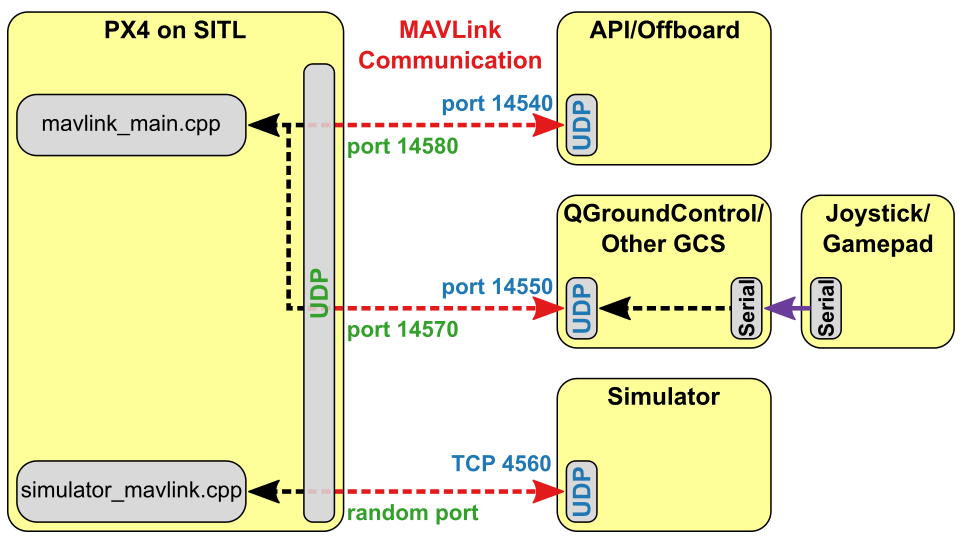
\includegraphics[width=\linewidth]{figures/px4_sitl_overview.png}
	\caption{PX4 kommunikációja Mavlink protokollal \cite{px4dev}}
	\label{fig:px4com}
\end{figure}

\section{Szimulációs környezet - Gazebo}
\begin{figure}
	\centering
	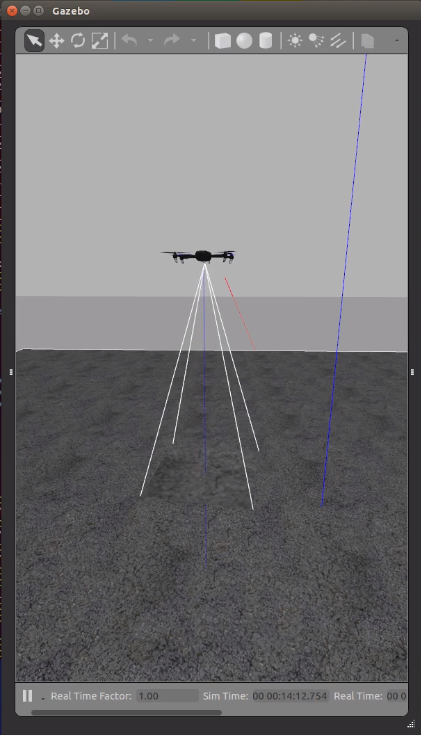
\includegraphics[height=12cm]{figures/sitl_optical_flow.png}
	\caption{Gazebo kamerás drón modell}
	\label{fig:sitl_optical_flow}
\end{figure}
Mivel a dolgozat egy nagy számú eszközkiszolgálást szeretne bemutatni és a tanszéknek egy Mantis Q drónja van, ezért a többinek a kiszolgálását szimulálni fogjuk, erre pedig kell egy szimulációs környezet, ami a Gazebo lesz. A Gazebo szimulátor lehetővé teszi az algoritmusok gyors tesztelését, a robotok tervezését, a regressziós tesztek elvégzését és akár AI rendszer kialakítását. Továbbá lehetőséget nyújt a robotok pontos és hatékony szimulálására komplex beltéri és kültéri környezetben. Kézhez kapunk egy 3D-s felületet is, amivel figyelni tudjuk a szimulációt, továbbá felhő alapú támogatást is biztosít, ami a témában még jól fog jönni.
A Gazebo különböző modelleket támogat, mint például a SITL optical flow, ami pont egy Mantis Q jellegű kamerás drónt szimulál bejövő és feldolgozható optikai adatcsomaggal (\ref{fig:sitl_optical_flow}. ábra). Az ábrán látható drónból kijövő fénykúp által vetődő keret lesz a kamera képe.
Sőt egy szimulált világba akármennyi modellt képesek vagyunk szimulálni a következőképpen.
\begin{lstlisting}[caption={10 optikai adatfolyamos drón szimulálása Gazebo-val}, label={lst:multi}]
cd src/Firmware
DONT_RUN=1 make px4_sitl_default gazebo
Tools/gazebo_multi_vehicle.sh -m sitl_optical_flow -n 10
\end{lstlisting}
\noindent
Az \ref{lst:multi}. számú listázásban futtatott script egyépként a szimulációs fájlrendszerben \emph{xacro} fájlokat módosítva éri el, hogy létrejöjjenek a kívánt modellek. Ezen a scripten könnyen lehet módosítani saját tetszésünk szerint. A modellek elérésének az UDP portjai 14560-tól, a TCP portjai 4560-tól inkrementálódnak, továbbá az összes a 14550 porton broadcast-el. \cite{multi-vehicle}

\noindent
A Gazebo felbontható szerverre és kliensre és a következő számításokat végzik:
\paragraph{Szerver}
\begin{itemize}
	\item Fizika kiszámítása
	\item Szenzorok szimulálása
	\item Engine API
\end{itemize}
\paragraph{Kliens}
\begin{itemize}
	\item Renderelés
	\item GUI
\end{itemize}

\section{Együttes működés}
A következő roslaunch utasítás egy lokális szimulációt indít a ROS-t összekötve MAVROS-al a \ref{fig:px4com}. ábrán látható módon keresztül.
\begin{lstlisting}[caption={Lokális PX4 szimuláció ROS-on keresztül Mavlink-el összekötve}]
roslaunch mavros px4.launch fcu_url:="udp://:14540@127.0.0.1:14557"
\end{lstlisting}
A szimulált világban való videót a QGroundControl alkalmazással lehet megfigyelni, továbbá akármennyi modell manuális irányítását is ezzel az eszközzel teszteltem. Persze a későbbi tömeges szimulációhoz, majd valamilyen automatizmusra lesz szükség. Az együttes működéshez szükséges egyfajta proxy, a mavlinken keresztül való kommunikációhoz, ami a Mavros (\ref{fig:egyuttes}. ábra).

\begin{figure}
	\centering
	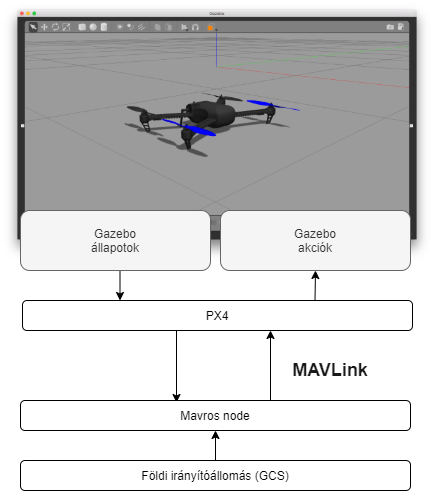
\includegraphics[height=10cm]{figures/egyuttes.png}
	\caption{Az együttes működés kommunikációja Mavros node-on keresztül}
	\label{fig:egyuttes}
\end{figure}
\chapter{Virtuális gépen kialakított tesztrendszerek}
A felhőberendszerbe való integrálás előtt két tesztet végzek Ubuntu VM-eken, amik a működés szempontjából fontosak lesznek.
\section{Azonos konténerrel egy drónvezérlés}
Az első ilyen teszt egy a TMIT tanszék egyik előre készített konténerével lesz, ez a DockerHub-on megtalálható \emph{bmehsnlab/aruco\_detect\_image\_v2} konténer. Ebbe a konténerbe bele van építve a videó stream, a kép feldolgozása, ami aruco kódokat detektál, a Mavros node működése és az irányító program.
Ezen konténerek indítása előtt ki kell adnunk az \emph{xhost} parancsot, mivel az X szerveren keresztül kommunikálnak egymással. Az X szerver kommunikációjához a konténereknek felcsatoljuk a \emph{/tmp/.X11-unix} fájlt.
\begin{lstlisting}[caption={Azonos konténerek indítása négy különböző feladattal és az X szerveren való kommunikációt megvalósítva}]
xhost +
docker run --net=host -v /tmp/.X11-unix:/tmp/.X11-unix --name stream bmehsnlab/aruco_detect_image_v2
docker run --net=host -v /tmp/.X11-unix:/tmp/.X11-unix --name dtctor bmehsnlab/aruco_detect_image_v2
docker run --net=host -v /tmp/.X11-unix:/tmp/.X11-unix --name mavros bmehsnlab/aruco_detect_image_v2
docker run --net=host -v /tmp/.X11-unix:/tmp/.X11-unix --name cntrol bmehsnlab/aruco_detect_image_v2
\end{lstlisting}
\begin{figure}
	\centering
	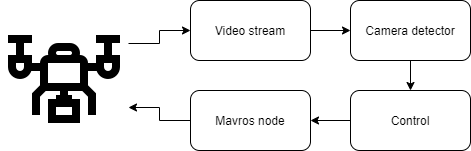
\includegraphics[width=\linewidth]{figures/local.png}
	\caption{Négy azonos konténerrel drónirányítás}
	\label{fig:azonos}
\end{figure}
A teszt architektúrája a \ref{fig:azonos}. képen látható. A teszt sikeresnek mondható, mivel a drónt sikerült irányításra bírni, illetve az optikai adatfolyamot fel tudta dolgozni az aruco kódfeldolgozó, habár aruco kódok nem voltak a szimulált világban.

\section{Két VM-en több drón szimulációja és vezérlése}
A következő teszten egy host OS-ből indított két VM-en teszteltem a több drón irányítását manuálisan. A teszthez telepítettem a VM-eken a fejezetben már felsorolt szoftvereket és környezeteket és a \ref{lst:multi}. listázásban bemutatott módon több drónt szimulációt is indítottam egy VM-en. Majd ezeket a földi irányítóállomás szimulátorával manuálisan vezéreltem. A teszt architektúrája a \ref{fig:ketvm}. ábrán látható.
\begin{figure}
	\centering
	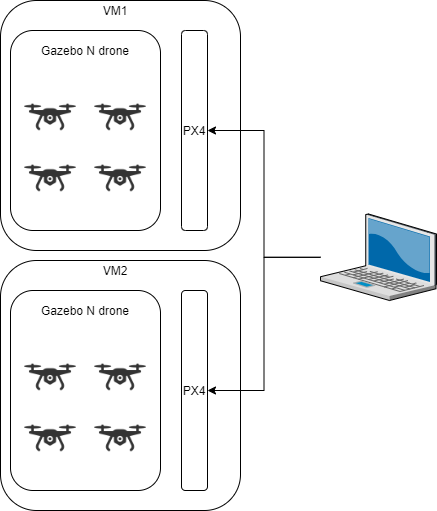
\includegraphics[height=10cm]{figures/multi-control.png}
	\caption{Két VM-en több drón irányítása}
	\label{fig:ketvm}
\end{figure}

\chapter{QoS sztohasztikus becslése}
\label{cha:toki}
A diplomaterv feladatai közé tartozik a Quality of Service (QoS), azaz a szolgáltatás minőségének a biztosításának megvalósítása, továbbá az 5G feltételrendszerével a feladat áttekintése.
\begin{figure}
	\centering
	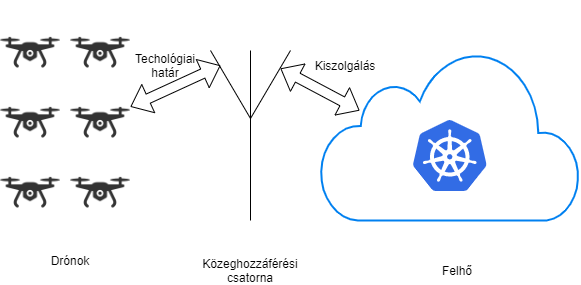
\includegraphics[width=\linewidth]{figures/qos.png}
	\caption{Több robot kiszolgálásának felhőből a durva modellje}
	\label{fig:qos}
\end{figure}
Egy durva modellben (\ref{fig:qos}. ábrán látható), a robotok felhővel való kiszolgálásának késleltetését két helyen vizsgálhatjuk:
\begin{enumerate}
\item Van egy technológiai határ, amit a nagy eszközszám kommunikációja határoz meg, ez annak a határa, hogy hány eszköz tud stabilan kommunikálni egy hálózaton, például az egyetem hálózatán. Tudjuk, hogy a Bluetooth, IEEE 802.11 különböző változatai és az LTE is más-más eszközmennyiséget tud kiszolgálni egyszerre egy antennán keresztül. Ebben a fejezetben ennek a limitációnak a kibővétéséről nem fog szó esni, de későbbiekben megnézzük, hogy mit tehet ennek a kibővítésnek az érdekében az 5G technológia.
\item A másik a felhő kihasználtsága és feladatelvégzési ideje. Itt a felhő feladatokat kap sorban valamilyen intenzitással és ezeknek a feladatoknak van egy elvégzési ideje, nyilván a Kubernetes cluster kapacitásának függvényében. Nyilvánvaló, hogy a felhő kihasználtsága valamilyen függőségben lesz a kiszolgálás idejével, ami a QoS-t meghatározza. Ebben a fejezetben azt a határt nézzük meg, hogy hogyan tudjuk méretezni a felhőnket, hogy valamilyen $t_0$ felsőbecsléssel élhessünk egy drón kiszolgálásának idejére, természetesen miliszecundumban.
\end{enumerate}

\section{Tömegkiszolgálási modell}
Valamennyi $R$ drón valamilyen $\lambda$ [kérés/s] intenzitással fordul a felhőhöz, hogy az számítást végezzen a kameraképen és megmondja mit kell csinálni. Erre a drón valamennyi idő múlva választ kap és ennek nem lehet a késleltetés értékét jelentősen megnövelni. A megbecsléséhez majd meg kell mérnünk, hogy átlagosan egy ilyen kérést a felhő mennyi idő alatt végez el, ez legyen $\mu$.
Feltételezhetjük, hogy nagy $R$ drónszám esetén függetlenül érkeznek a kérések, így modellezhetünk Poission folyamattal a beérkező kéréseket nézve. Tehát ha egy drónnak a kérési intenzitása valamilyen feladatra $\frac{\lambda}{R}$, akkor az összes drónnak $\lambda$.
Ezt tekinthetjük egy Markov folyamatnak, ahol az infinitezimális generátorból tudunk majd valamilyen sorhossz várhatóértékeket kiszámítani. Mivel nem vesznek el kérések, csupán torlódik a sor, ezért ez egy M/M/1 kiszolgálási modell. \cite{toki}
Az infinitezimális generátor definíció szerint
\[ G =
\begin{bmatrix}
-\lambda & \lambda & 0 & 0 & 0 & 0 & ... \\
\mu & -(\lambda+\mu) & \lambda & 0 & 0 & 0 & ... \\
0 & \mu & -(\lambda+\mu) & \lambda & 0 & 0 & ... \\
0 & 0 & \mu & -(\lambda+\mu) & \lambda & 0 & ... \\
0 & 0 & 0 & \mu & -(\lambda+\mu) & \lambda & ... \\
: & : & : & : & : & : & .
\end{bmatrix}
\]
Ami annyit mond, hogy a várakozó eszközök sorhossza $\lambda$ intenzitással növekedik egyet, amikor érkezik egy kérés és $\mu$ intenzitással csökken egyet, amikor elvégződik egy kérés.

\section{Várakozási idő várható értéke}
Ha a tömegkiszolgálási modellünk jó és tényleg tekinthetjük a kérések eloszlását egy véletlennek, amit nem nagyon specifikus drónirányítás esetben megtehetünk, akkor egy M/M/1-es rendszer kiszolgálási késleltetését kell megnéznünk. A \cite{toki} jegyzet 4.4-es fejezet bebizonyítja,ennek a modellnek a késleltetését, ami a drón kérésére visszakapott válasz a felhő és az antenna között a $D$ késleltetéssel arányos. A jegyzet bizonyítása alapján: \[ D = \frac{1}{\mu - \lambda} \]


\chapter{Kialakított Kubernetes alapú felhő}
\label{cha:kubernetes}

Ebben a fejezetben rátérünk a felhőrendszer tényleges megvalósítására. A \ref{cha:cloud}. fejezetben megnéztük milyen lehetséges mai technológiák közül választhatunk, realizálhattuk, hogy a Kubernetes tűnik a legjobb választásnak ilyen célra, most pedig ezen a vonalon haladunk tovább. Megnézzük Kubernetesen belül milyen lehetőségek vannak, mik a probléma alapfeltételei és hogyan lehet integrálni a \ref{cha:fizikai}. fejezetben bemutatott konténerkollaborációt egy ilyen Kubernetes felhőbe.

\section{Kubernetes technológiái}
Több Kubernetes technológia közül választhatunk, bepillantunk némelyikbe, hogy mire jó és miért ezt választjuk vagy nem választjuk.

\subsection{K8S}

A K8s a Kubernetes rövidítése ("K", majd 8 "ubernete", majd "s" betű). Azonban általában, amikor az emberek Kubernetesről vagy K8-ról beszélnek, akkor az eredeti upstream projektről beszélnek, amelyet a Google valóban rendkívül elérhető és skálázható platformként tervezett.

Tehát a Kubernetes minden alapfunkcióval, mely összességének tulajdonságai:
\begin{itemize}
	\item elválasztott Master és Worker node-ok, biztosítható az irányítás erőforrása
	\item etcd külön clusteren futtatható, biztosítható a terhelés kezelése
	\item ideális esetben külön bejáratú csomópontokkal rendelkezik, hogy azok könnyedén kezeljék a bejövő forgalmat, még akkor is, ha az alatta lévő csomópontok némelyike foglalt. \cite{k8svsk3s}
\end{itemize}
\subsection{K3S}
A K3S egy egyszerűsített változata a K8S-nek, melynek forrása 40MB bináris fájl, amely teljesen implementálja a Kubernetes API-t. Rengeteg extra driver-t kihagytak belőle, melyre alap esetben nincs szükség tesztrendszer vagy egyszerű klaszter esetén. Ezeket a kihagyott funkciókat egyébként később hozzá lehet illeszteni a rendszerhez add-onokkal. \cite{k8svsk3s}
\subsection{Kind}

A Kind egy Docker fölötti Kubernetes megvalósítás egy node-on. Egyszerű installálni, azonban nem a Kubernetes API-t használja.

\subsection{MiniKube}

A MiniKube az első Kubernetes technológia amely a fejlesztők ajánlása alapján a kezdőknek kipróbálásra a legalkalmasabb. Mivel egyszerű telepíteni, nincs nagy erőforrásigénye (2 vCPU/2GB RAM/20GB lemez). Egy gépre installálható, nem adható több node a klaszterhez. \cite{typesofkubernetes2}

\subsection{Miért K3S?}

A tanszéki klaszter természetesen egy teljes kialakított K8S, melyen az eredeti API használható és teljesértékű szolgáltatásokat lehet tesztelni a Kubernetes összes optimalizálásával. A Kind más API-t használ, így a telepítést leegyszerűsíteni, azonban nem összeegyeztethető egy Kind-os applikáció K8S megvalósításával. MiniKube már egyel jobb, azonban csak egy node-ot használ, ebben a projekben pedig fontos a hálózati tesztelés több node között. Így marad a K3S, amellyel a legjobban szimulálhatjuk a tanszéki K8S rendszert és a megvalósított applikáció is könnyen portolható.

\section{Földi scenario felkészítése a menedzselt felhőrendszerbe}

A felhasznált Docker konténereket néhány esetben változtatni kellett, ez csak a \emph{Dockerfile}-ra igaz, a forráskódok az eredeti esetben is működtek nem K3S rendszeren. Mindegyik konténerben volt egy kivétel, amely csak akkor engedte futtathatóvá tenni a konténert, ha az Docker rendszerben fut, ezt a \emph{[/.dockerenv} fájl létezésére vonatkozó feltétel. \\

\noindent
A PX4 szimuláció futtatószkripje (\emph{vke\_px4sim/docker-entrypoint.sh}) ugyan tartalmazza a beépített \emph{ROS\_IP} hirdetőcímet, amelyet a hálózati fejlesztés során többször átírtam, sikerült olyan végeredményre jutni, amelyben az eredeti konténer külső interfész IP-je maradhat. \\

\noindent
Az előkészített Roscore konténert a végleges verzióban nem használom, hiszen egyszerűbb volt az eredeti \emph{alpineros/alpine-ros:noetic-ros-core} publikus image-t megadni, amit a K8S API-ban tudtam testreszabni indított portszámmal és környezeti változókkal.

\section{Kubernetes virtualiztált telepítése Multipass VM-eken}

Egy több node-os klasztert valósítok meg virtualizáció fölött. Virtuális gépek létrehozására rengeteg program létezik, én a Multipass-t választottam. A Multipass egy letisztult VM menedzser Linux-ra, Windows-ra és MacOS-re, amellyel egy parancs indítani és törölni különálló VM-eket bármely CloudInit-et tartalmazó image-ről. Azért választottam ezt, mert könnyedén szkriptelhető a Klaszter törlése és felhúzása, mivel a fejlesztés során sokszor szeretném az alapbeállításról indítani a klasztert. \\

\noindent
Tehát írtam egy Bash scriptet, aminek segítségével létrehozok három VM-et és inicializálom rajtuk a K3S klasztert. Multipass VM-ek létrehozása Bash-ben egy-egy parancs (\ref{lst:mlaunch}. számú lista), melyek paramétereit természetesen egy config fájlból olvasok be, amiről még később szó lesz.
\begin{lstlisting}[caption={Multipass VM-ek létrehozása},label={lst:mlaunch}]
multipass launch --name master --cpus 2 --mem 2G --disk 2G
for w in "worker-1 worker-2"; do
	multipass launch --name $slave --cpus 2 --mem 2G --disk 30G
done
\end{lstlisting} 
\noindent
Létrehozás után a szkript kiadatja az Apt csomagkezelő program \emph{update és upgrade} parancsait, hogy a legfrissebb Ubuntu 20.04 kompatibilis csomagok legyenek a VM-eken. \\

\noindent
Frissítés után a master VM-en inicializálható a K3S master módban. A parancs eleje azt mutatja, hogy a master nevű VM-en hajtjük végre a "--" utáni parancsokat (\ref{lst:minit}. lista).
\begin{lstlisting}[caption={K3S Master inicializálása},label={lst:minit}]
multipass exec master -- /bin/bash -c "curl -sfL https://get.k3s.io | K3S_KUBECONFIG_MODE="644" sh -"
\end{lstlisting}
\noindent
Ha ez sikeres, akkor a worker node-okat is inicializálhatjuk, amihez két dologra lesz szükség, a master külső IP-jére, amin keresztül a másik VM tudja elérni, illetve a K3S egyedi tokenre. A master külső IP-jét a multipass egyik parancsából olvassuk ki, a grep programmal rákeresve a master névre, majd az IP cím formátumára reguláris kifejezéssel. A tokenhez szimplán kiíratunk egy fájlt a cat programmal. Ezekkel pedig a master-hez hasonló módon a K3S dokumentációban megadott curl programhívással inicializáljuk a slave-eket. (\ref{lst:initk3s}. lista)
\begin{lstlisting}[caption={K3S Slave-ek inicializálása},label={lst:initk3s}]
K3S_TOKEN=$(multipass exec $master sudo cat /var/lib/rancher/k3s/server/node-token)
MASTER_IP=$(multipass list | grep $master | grep -oE "\b([0-9]{1,3}\.){3}[0-9]{1,3}\b")

for slave in $slaves; do
	multipass exec $slave -- /bin/bash -c "curl -sfL https://get.k3s.io | K3S_TOKEN=${K3S_TOKEN} K3S_URL=https://${MASTER_IP}:6443 sh -"
done
\end{lstlisting}

\noindent
Sikerességet ellenőrizve a szkiptben még kiíratom a master-en a csatlakozott node-okat.
\begin{lstlisting}[caption={Node-ok lekérdezése}]
multipass exec $master kubectl get nodes
\end{lstlisting}

\section{Konténer registry, lokális és központi}
Docker-Compose esetén a konténer kollaborációs megvalósításhoz elég volt definiálni a könyvtárt, mely forrása és konfigurációja alapján meg kell építeni az image-et és a lokális Docker környezet eltárolta ezen image-eket, amit fel is tudott használni az adott környezetben. Ez természetesnek tűnt, azonban a Kubernetes alapvetően nem tartalmaz ilyen fejlesztéseket, csakis lefordított képfájlokat tud publikus vagy privát registry-ből letölteni. A Docker Registry egy olyan verziókezelő, amely felépített konténer képfájlokat tárol és állít rendelkezésre aktívan használó rendszereknek, mint például a Kubernetes vagy Docker Swarm. Három megoldást próbáltam ki, hogy az egyedi lemezképeket használhassam a felhőmben (\ref{fig:registry}. ábra).\\

\noindent
\paragraph{A)}
Elsőnek úgy gondoltam, hogy a legegyszerűbb megoldás az ha a K3S vagy egy Docker környezetben, amely a K3S master-én futna, inicializálok egy előre készített Docker registry szervert, arra feltöltöm a felépített konténerlemezeket és lokálisan eléri a Kubernetes master, deploy esetén. Tehát definiáltam egy pod-ot, amely az 5000-res porton elérhető a K3S rendszeren belül, a master-ről. A \emph{registry} nevű image-et adtam meg, így a hivatalos Docker registry került letöltésre. Push-olni sikerült konténert, azonban a Kubernetes API-ra definiált Deployment-el már nem sikerült pull-olni SSL biztonsági okok miatt. \\

\noindent
\paragraph{B)}
Ezután hagytam a felhőbe integrálást, a master node-ra telepítettem Dockert és Docker-Compose-t, majd a deploy-oltam a hivatalos oldalról a registry-t (\ref{lst:registryB}. lista). A konténerek push-olása pedig szintén a master node-ról történt (\ref{lst:localreg} lista). Ez a megoldás működött, azonban nem túl szép és optimális, mivel a master-en sokszor tárolódik egy konténer image (forrásként, Docker image-ként, Docker registry-ben, Kubernetes letöltött image-ként és példányosított konténerként).
\begin{lstlisting}[caption={Docker registry inicializálás a master docker környezetében},label={lst:registryB}]
multipass exec ${master} -- sudo docker run -d -p 5000:5000 --restart=always --name registry registry:2
\end{lstlisting}
\begin{lstlisting}[caption={Build és push lokál konténer registry-be},label={lst:localreg}]
for container in "commander px4sim aruco"; do
	multipass exec ${master} -- sudo docker build ${drone_control_dir}/vke_${container}/. -t localhost:5000/${container}
	multipass exec ${master} -- sudo docker push localhost:5000/${container}
done
\end{lstlisting}

\paragraph{C)}
Így inkább talán a legegyszerűbb megoldást választottam, igénybe vettem a hivatalos Docker Hub privát repository szolgáltatását, amely ugyan egy konténert biztosít ingyen, egy kis trükkel, mi szerint ugyanazt a konténert töltöm fel 3 különböző taggel, ezt is meg lehet oldani (\ref{lst:registryC}. lista).
\begin{lstlisting}[caption={Docker Hub build és push},label={lst:registryC}]
for container in "commander px4sim aruco"; do
	docker build ${drone_control_dir}/vke_${container}/. -t nanasidnl/drone_control:${container}
	docker push nanasidnl/drone_control:${container}
done
\end{lstlisting}

 \begin{figure}
 	\centering
 	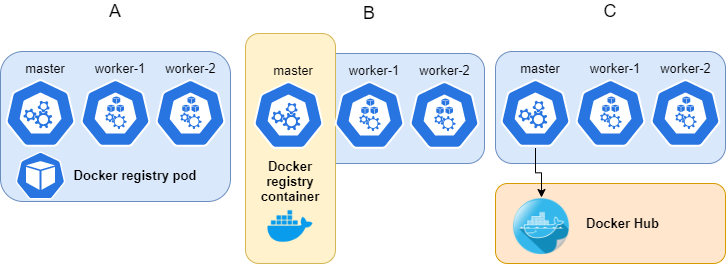
\includegraphics[width=\linewidth]{figures/registry.png}
 	\caption{Registry megoldásaim egyedi konténerek esetén}
 	\label{fig:registry}
 \end{figure}

\noindent
A Docker Hub privát repository-hoz authentikálni kell az API-t, ahhoz hogy elérje az adott K8S deployment. Ehhez egy configurációs fájlba kiszerveztem a hitelesítő adatokat. A szolgáltatást létrehozó deploy szkriptbe pedig beleírtam, hogy használja fel ezt a fájlt és authentikáljon egy \emph{regcred} titkon keresztül (\ref{lst:dhk3s}. lista). Ezt meg kell adni az API használatakor is (\ref{lst:dhsec}. lista).
\begin{lstlisting}[caption={Docker Hub authentikáció K3S-ről},label={lst:dhk3s}]
source ../config/docker-credentials.sh
multipass exec ${master} -- kubectl create secret docker-registry regcred --docker-server=${docker_server} --docker-username=${docker_username} --docker-password=${docker_password} --docker-email=${docker_email}
\end{lstlisting}

\begin{lstlisting}[caption={K8S API secret definiálása a konténerekhez},label={lst:dhsec}]
imagePullSecrets:
- name: regcred
\end{lstlisting}


\chapter{Drónirányítás mint szolgáltatás a Kubernetes felhőben}

Az előző (\ref{cha:kubernetes}.) fejezetben megmutattam, hogyan alakítottam ki a saját felhőrendszeremet. Ebben a fejezetben pedig megnézzük a diplomamunkának szánt feladat miként tud felkerülni ebbe a felhőbe.

\section{Első, 4 podos megvalósítása a szolgáltatásnak}
Elsőként a legegyszerűbb összeállításban szerettem volna megbizonyosodni arról, hogy a szolgáltatás valóban tud működni a felhőben ezért elsőnek a négy konténert 4 különálló pod-ként próbáltam ki (\ref{lst:1pod4}. lista). \\

\noindent
A Pod a legkisebb telepíthető számítási egység, amely létrehozható és kezelhető a Kubernetesben. Egy Pod létrehozása esetén példányosodik az előre definiált konténer vagy konténer csoport, azonban a futás megkezdése után semmilyen felügyeleti szolgáltatásban nem részesül, nem indul újra leállás esetén, nem alkalmazódik rá semmilyen skálázás. Egyszerűen ha csak Pod szinten futtatunk alkalmazásokat, akkor ugyanott járunk mintha Docker Swarm környezetben dolgoznánk. \\
\begin{lstlisting}[caption={Példa egy Pod-ra a négyből},label={lst:1pod4}]
apiVersion: v1
kind: Pod
metadata:
	name: aruco
	labels:
		name: drone-hq
spec:
	hostname: aruco
	containers:
	- 	image: nanasidnl/drone_control:aruco
		name: aruco
	env:
	- 	name: ROS_MASTER_URI
		value: "http://roscore:11311"
	- 	name: ARUCO_LAUNCH
		value: "sim"
	imagePullSecrets:
	-	name: regcred
\end{lstlisting}

\noindent
Jelen négy Podos megvalósításban a belső hálózati problémák nem merültek fel, hiszen a Pod neve hostname-ként is funkcionál, így egymás között könnyedén el tudták érni egymást az alkalmazások. Ez egy működő verzió volt, azonban túl egyszerű. A drón szimulációt nem a felhőben képzeljük el, hiszen a fizikai drón sem a felhőben fog futni.

\section{Konténerek hálózata, service-deployment 1 podos megoldás}

\section{Load Balancer, NodePort, Ingress}
https://medium.com/google-cloud/kubernetes-nodeport-vs-loadbalancer-vs-ingress-when-should-i-use-what-922f010849e0

\section{ROS Port forwarding}
https://journals.sagepub.com/doi/pdf/10.1177/1729881417703355

\section{Kauzalitási probléma, deploy sorrend}

\section{N drónra K3S service és drónok deployolása}

\section{N drón irányítása K3S-ből}

\chapter{Drónkapcsoló állomás Kubernetes felhőben}
Ebben a fejezetben, a kialakított K3S alapú drón kiszolgáló központot fejlesztem tovább, úgy hogy valamilyen QoS feltételeket valósítson meg. Megnézzük, hogyan választottam technológiát a szoftver architektúráját, részleteit. Tárgyaljuk, hogy milyen architekturális változást kell végeznünk ahhoz, hogy javítsuk a válaszidőt. Megmutatom a Node váltási lehetőségeket és becsléseket teszek a hatékonyságukra. \\

\noindent
A fejlesztendő szoftver a drón közelébe tervezett, tehát nem a felhőben fog futni, hanem a drónok központi irányításának a kiegészítése. E szerint futtatását azon a gépen célszerű végezni, mely a drónnal is egy hálózaton/környezetben van.

\section{Felhasznált technológia}
Olyan technológiában kell megkezdeni a fejlesztést, amely lehetőséget biztosít egyszerű kezelésére az eddig felállított rendszernek és környezetnek. Szükséges belevinni modularitást és sklázhatóságot, továbbfejlesztési lehetőség érdekében. Tehát a felhasználó számíthat rá, hogy nagyobb számú drón vagy robotvezérlést is támogat a rendszer. \\

\noindent
Mivel egy QoS megvalósításáról beszélünk, amelynek paraméterei változhatnak a szükségletek függvényében, ezért az implementáció részeként csak a logikai működést szükséges megvalósítani, az egyes kritériumok változtathatóak. A bevezetőben szó esett különböző jövőbeli automatikus drónfelhasználásnak, melyben volt példa élő szórakoztatóipari fellépésre és mezőgazdasági munkára is. Ezen iparágakban teljesen más QoS feltételeket szabnak meg. Míg egy élő fellépésben nagyon hamar belerondíthat a show-ba pár késleltetésből félreszinkronizált drón, addig a mezőgazdaságban inkább hosszú idejű stabilitásnak kellhet megfelelni. Ezért az algoritmus megalkotásánál paraméterekben fogunk dolgozni, melyeket a felhasználás definiál.

\subsection{Vezérlést megvalósító programozási környezet}
A szakmai előítéleteim alapján már sejtettem, hogy a Python lesz az a nyelv, amelynek a legtöbb támogatása van a natív felhőtechnológiákhoz. A Python egy értelmezett, magas szintű és általános célú programozási nyelv. A Python tervezési filozófiája hangsúlyozza a kód olvashatóságát a jelentős szóköz jelentős felhasználásával. Nyelvi konstrukcióinak és objektum-orientált megközelítésének célja, hogy segítsen a programozóknak világos, logikus kódot írni kis és nagy projektekhez. A Python dinamikusan be van írva és automatikus garbage-collector-ral működik. Támogatja a több programozási paradigmát, beleértve a strukturált (különösen az eljárási), az objektum-orientált és a funkcionális programozást. A Python-t átfogó szabványos könyvtárának köszönhetően gyakran "csomagokkal együtt" használt nyelvként írják le. \cite{pwiki} \\

\noindent
Amely lehetőségek miatt kifejezetten a Python technológiát választottam azok az alábbiak:
\begin{itemize}
	\item Kubernetes API támogatás
	\item Docker API támogatás
	\item Könnyű naplózás, időalapú feljegyzés
	\item Gyenge objektumorientált támogatás, a modularitás és a tiszta kód miatt
	\item Egyszerűség, gyengén típusosság
\end{itemize}

\noindent
A dolgozathoz mellékelt könyvtár \emph{switchingCenter} nevű könyvtárban található a Python projekt implementáció. A könyvtárban található még egy \emph{requiments} felsorolás, mely a használt Python könyvtárakat sorolja fel azzal a verzióval, mellyel teszteltem is. Ezen kiegészítések telepítése a Pip programmal lehetséges az adott környezetben (\ref{lst:pip}. kódrészlet).

\begin{lstlisting}[caption={Python könyvtárak telepítése}, label={lst:pip}]
pip install - r requiments.txt
\end{lstlisting}

\noindent
A programhoz tartozó beállításokat egy globális fájlba helyeztem, melyet a Bash és a Python program egyaránt fel tud használni, utóbbi a \emph{ConfigObj} konfiguráció illesztő modullal.

\subsection{Kubernetes könyvtár alkalmazása}
Nyílt forráskódú, stabil verziójú Kubernetes Python kliens létezik, amelyet felhasználtam a fejlesztés során. \cite{kubpy} Mint a kliens főoldalán is látható, Kubernetes API-t széleskörűen támogatja, így az általam felhasznált Kubernetes API technológiákat is. \\

\noindent
A jelenlegi környezetben a program felhasználja a Multipass program parancsait a Bash-en keresztül, ami nem túl kifinomult mérnöki kivitelezés, azonban a Multipass-nak még nincs Python kliense, illetve későbbi rendszerek esetén könnyen átfejleszthető másra. A külső program meghívására a \emph{subprocess} modult használtam, mely segítségével kértem le a master VM-ről a K3S tokent és a master IP-jét. Utána a kapott információkból fel tudtam építeni a Kubernetes authentikációt, megadva a Multipass által generált privát kulcsot is (\ref{lst:kubclient}. kódrészlet).

\begin{lstlisting}[caption={Kubernetes kliens felépítése}, label={lst:kubclient}]
aToken= subprocess.check_output(["multipass", "exec", self.config_parser.get('master'), "--", "kubectl describe secret $SECRET_NAME | grep -E '^token' | cut -f2 -d':' | tr -d " ")"]).decode('utf-8')
master_ip= subprocess.check_output(["multipass", "list", "|", "grep", self.config_parser.get('master'),'grep -oE \b([0-9]{1,3}\.){3}[0-9]{1,3}\b']).decode('utf-8')

aConfiguration = kubernetes.client.Configuration()
aConfiguration.verify_ssl = False
aConfiguration.host = "https://"+master_ip+":443"
aConfiguration.api_key = {"authorization": "Bearer " + aToken}
aApiClient = kubernetes.client.ApiClient(aConfiguration)

self.kApi = client.CoreV1Api(aApiClient)
\end{lstlisting}

\subsection{Docker könyvtár alkalmazása}
A \emph{Docker SDK for Python} segítségemre volt, hogy a Drónokat elérjem és parancsokat adhassak ki a konténeren belül. Az SDK nagyon egyszerű lehetőséget nyújtott kapcsolódni a környezethez, kifejezetten ha a szoftver is ugyanabban a fut. \\

\noindent
Definiáltam egy Drone osztályt, amely példányosításával egy drónhoz kapcsolódik a program, melyet tárol és fenntartja a kapcsolatot. Az inicializálás a drón száma alapján történik, hasonlóan a korábbiakhoz, az azonosítóból kiszámoljuk a portokat, mely kezdőportokat a konfigfájlból olvasunk ki (\ref{lst:droneconnect}. kódrészlet). A konténert a konvencionális nevezéktanon keresztül ismerjük fel (drone-1, drone-2, ...), mely konténer lekérése után bármilyen Docker parancsot végre tudunk hajtani a \emph{self.drone} elnevezésű kliens segítségével.

\begin{lstlisting}[caption={Drón konténeréhez csatlakozás}, label={lst:droneconnect}]
class Drone():
	def __init__(self, drone_id, node_ip):
		self.config_parser = ConfigObj('../config/config')
		self.drone_id=int(drone_id)
		self.node_ip=node_ip
		self.docker_client = docker.from_env()
		self.mavlink_port = int(self.config_parser.get('MAVLINK_START_PORT'))+drone_id-1

		self.drone= self.docker_client.containers.get("drone-"+str(self.drone_id))
\end{lstlisting}

\subsection{Naplózás}
Szoftveremben nagyon fontos a naplózás, melyet a \emph{logger} modullal valósítottam meg. A QoS miatt minden egyes tevékenységet, amit a program elvégez nyers időbélyeg formátumban írom ki, hogy méréseket lehessen végezni a tevékenységek között (\ref{lst:logconf}. kódrészlet).

\begin{lstlisting}[caption={Naplózás beállítása}, label={lst:logconf}]
logging.basicConfig(filename='switchCenter.log', level=logging.INFO, format='%(asctime)s %(levelname)-8s %(message)s')
\end{lstlisting}

\section{Kivitelezési lehetőségek és várható kapcsolási idők}

Tehát van egy automatizáltan felépített rendszerünk Kubernetes-szel és változtatható mennyiségű szimulált drónnal. És már a szoftver is készen áll, hogy bármely automatizált szabályokat figyelhessünk és bármilyen módosítást végrehajtsunk valós időben a rendszeren. De mik is azok a feltételek, amelyek egy QoS biztosítanak egy ilyen drónokat irányító felhőrendszerben? Definiálom ezeket egy drónra:
\begin{itemize}
	\item A drón és a Kubernetes közötti válaszidő nem haladhat meg egy előre definiált maximális időt,
	\item A drón és a Kubernetes közötti sávszélesség nem lehet kisebb egy előre definiált minimális sávszélességnél, ez a sávszélesség szétbontható egy irányításra meghatározott biztonsági és egy videófolyam sávszélességre,
	\item Ha ezen feltételeknek nem felel meg az adott konstrukció, végezzen változtatást,
	\item Ha nem létezik olyan változtatást elvégezni, amellyel megfelelnek a feltételek, akkor érjen véget a program és jelezze, hogy véget ért a QoS feltételek melleti üzemelés, mely esetnen létrejöhet valamilyen biztonsági procedúra, például biztonságos leszállás.
\end{itemize}

\noindent
A következőkben megnézzük, hogy mi az a változtatás amivel javítani lehet a kapcsolaton. Jelen rendszerben egy 3 Node-os felhőrendszerről beszélünk, amely lehet sokkal szélesebb is, a K8S határain belül. Az implementációnál figyelembe vettem a változtatható Node mennyiséget. Ha valamilyen kritériumnak nem felel meg a kapcsolat, akkor egyféleképp változtathatjuk a kapcsolatot, áthelyezzük a háttérszolgáltatást másik Node-ra. Ebben a lokális virtuális rendszerben ez nem tűnik megoldásnak, de egy nagyobb ipari klaszter ezetén a távolságokból adódóan Node váltással érhetünk el jobb eredményt, biztosíthatjuk rendszerünket túlterheltség és véletlen hiba létrejötte esetén. Tehát akkor azt kell megnéznünk, mely módokon lehet kivitelezni.

\subsection{Node váltás és új címhirdetés}
Első ilyen megközelítés, hogy ha már automatizáltan fel tudjuk építeni a Roscore-t, akkor legyen a változtatás az, hogy új Node-ra deploy-oljuk a Roscore-t és közöljük a drónnal az új elérési címet. Nézzük meg mi ennek a pontos menete:
\begin{itemize}
	\item Észrevesszük a hibát és reagálunk ($t_{r}$)
	\item Kiválasztunk egy megfelelő Node-ot ($t_{s}$)
	\item Deploy-oljuk a Roscore-t az új Node-on ($t_{d}$)
	\item Új címet adunk meg a drónnak ($t_{a}$)
\end{itemize}
Összesen $t = t_r + t_s + t_d + t_a$ idő. Azt fontos megjegyezni, hogy a $t_r$ reagálási idő konfigurálható vagyis az, hogy milyen időközönként nézzük, amiből tudjuk, hogy a reagálási idő várható értéke az ellenőrzési periódusidő fele lesz.

\subsection{Node váltás proxy mögött}
Nézzünk meg egy másik megközelítést, amikor meg szeretnénk spórolni $t_a$ címadási időt és kihelyezünk egy proxy-t amely megváltoztatja a mögöttes Node-ot miután a Roscore-t deploy-oltuk az új Node-ra. A probléma továbbra is fennáll, hogy ha egy Node-on fut a Roscore, akkor azt kívülről az elérhető portok nagy részén el kell tudnunk érni. A Kubernetes Service API működhetne ilyen proxy-ként, azonban nem fogja biztosítani a többi portot LoadBalancer nélkül. Sima Kubernetes proxy-val azonban elméletben meg lehet oldani (lásd dokumentáció \cite{proxy}). Azonban ezzel a megoldással létrejönne a proxy kreálás/változtatás ideje, illetve az új proxy-n keresztül hitelesítést is kell végeznünk minden alkalommal. 

\subsection{Széleskörű rendelkezésre állás}
A legtöbb időt jelentő $t_d$ deploy időt, ami méréseim szerint 2 és 5 másodperc között van, akkor iktathatjuk ki, hogyha nem csak az aktív Node-on áll rendelkezésre az adott drónnak a Roscore, hanem legalább egy backup Node-on. Ezzel a verzióval ugyan átlagosan több erőforrást foglalunk, azonban optimalizálhatjuk a váltási időt, ami javít a QoS-en.

\section{Vezérlési podok telepítése}
Kiderült, hogy a legoptimálisabb QoS megoldása az lehet, ha minden worker Node-on rendelkezésre áll a Roscore minden drón számára. Ezt a DaemonSet Kubernetes API-val lehet megvalósítani. \\

\noindent
A DaemonSet biztosítja, hogy az összes (vagy néhány) Node futtassa a Pod másolatát. Amint  Node-ok hozzáadódnak a klaszterhez, a Podok automatikusan létrejönnek az új Node-okon. Amint a Node-okat eltávolítják, ezeket a Podokat a Kubernetes Garbage-Collectora gyűjti össze. A DaemonSet törlése megtisztítja az általa létrehozott Podokat. Egyszerű esetben minden démontípushoz egy, minden csomópontot lefedő DaemonSet-et használnak. A bonyolultabb beállítás több DaemonSet-et is használhat egyetlen démontípushoz, de különböző jelzőkkel és / vagy különböző memória- és CPU-kérelmekkel a különböző hardvertípusokhoz. \cite{daemonset} \\

\noindent
A Kubernetes Service API helyett használom a megvalósítandó ötletben a DaemonSet-et a következőképpen (\ref{lst:daemonset}. kódrészlet). A konténer indítás és a változók ugyanazok maradtak, mint a Service-es megvalósításban, az \emph{affinity} résszel egészítettem ki a yaml-t. Itt \emph{hostname} alapján szűröm ki a Node-okat, azokon a Node-okon fog elindulni a Roscore, melyek nem tartalmazzák a master nevet.

\begin{lstlisting}[caption={DaemonSet megvalósítás, Roscore minden worker-en}, label={lst:daemonset}]
apiVersion: apps/v1
kind: DaemonSet
metadata:
	name: roscore-$(DRONE_IDENTIFIER)
spec:
	selector:
		matchLabels:
			app: roscore-$(DRONE_IDENTIFIER)
	template:
		metadata:
			labels:
				app: roscore-$(DRONE_IDENTIFIER)
		spec:
			affinity:
				nodeAffinity:
					requiredDuringSchedulingIgnoredDuringExecution:
						nodeSelectorTerms:
						-	matchFields:
							-	key: metadata.name
								operator: NotIn
								values:
								-	master
			hostname: roscore-$(DRONE_IDENTIFIER)
			containers:
			-	name: roscore-$(DRONE_IDENTIFIER)
				image: alpineros/alpine-ros:noetic-ros-core 
				env:
				-	name: ROS_IP
				valueFrom:
					fieldRef:
						fieldPath: status.podIP
			-	name: ROS_MASTER_URI
				value: "http://$(ROS_IP):$(MAVLINK_PORT)"
			args: ["roscore", "-p", "$(MAVLINK_PORT)"]
		hostNetwork: true
\end{lstlisting}

\section{Mérési adatok kinyerése}
A rendszer automatikus működéséhez szükséges megtudnunk az aktuális sávszélességet és válaszidőt a drón és a node között. Mivel a szoftver a drón közelében fut, ezért a jelenlegi szimulált rendszerhez implementálom, azonban ezek a függvények változtathatóak lesznek. A program a konténerből tud kiadni alap Linuxos parancsokat, így a sávszélességet iperf programmal (\ref{lst:bw}. kódrészlet), a válaszidőt ping programmal (\ref{lst:ping}. kódrészlet)  nyertem ki. Ha nem sikerülne elvégezni a program futását, akkor visszatér egy magas értékkel, melyet lemér mégegyszer a váltás előtt. Ping esetén eldönthetjük, a függvény paraméterében, hogy hány ICMP packet átlagát szeretnénk venni.

\begin{lstlisting}[caption={Sávszélesség megállapítása a konténer és a node között}, label={lst:bw}]
def getBW(self, node_ip):
	iperf="iperf3 -f m -c "+node_ip
	(exit_code,output)= self.drone.exec_run(iperf)
	outputStr = output.decode('utf-8')
	try:
		return float(outputStr.split('\n')[-1].split(' ')[4])
	except:
		return 10000
\end{lstlisting}

\begin{lstlisting}[caption={Késleltetés megállapítása a konténer és a node között}, label={lst:ping}]
def getConnectionDelay(self, node_ip, n=1):
	pingCommand="ping "+node_ip+" -c "+str(n)
	(exit_code,output)= self.drone.exec_run(pingCommand)
	outputStr = output.decode('utf-8')
	for line in outputStr.split('\n'):
		if 'min/avg/max/mdev' in line:
			avg=line.split('/')[5]
			return float(avg)
	else:
		return 10000
\end{lstlisting}






\chapter{Távoli Robotvezérlés Optimalizálása}
\label{cha:alg}

Ebben a fejezetben a távoli robotvezérléshez használt algoritmust ismertetem. Az algoritmus célja, hogy a drónok vezérléséhez biztosítsa a QoS feltételeit, amit jelen esetben két paraméterben határozunk meg: sávszélesség és válaszidő. Ennek a két paraméternek a kontrollálásával biztosítható a videó folyam minősége a drón és a Kubernetes Node-ok között. A Kubernetes klaszter worker node-jai (rendelkezésre álló szerverek) erőforrás készletének függvényében a videófeldolgozás és a drón irányítása áthelyezhető (váltható, migrálható) az optimális teljesítmény érdekében. Az algoritmus rendszeresen méri az elérhető erőforrásokat, proaktívan vált a szolgáltatás zökkenőmentes fenntartása érdekében. \\

\noindent
Tehát van valamennyi Node-unk amik között a drónok vezérlését áthelyezhetjük, az algoritmus úgy vált időközönként, hogy a késleltetést optimalizálja és biztosítja a sávszélességet is. Ha a sávszélességet nem lehet biztosítani, akkor egy ALARM állapotba fut, ekkor a drón biztonságosan leszáll és azonnal értesíti a felhasználót. \\

\noindent
Az algoritmus bemenete tehát a Node-ok IP címének halmaza, amin keresztül kapcsolódik a drón a központhoz, a minimum sávszélesség a videó folyamra felé (vbw), a minimum sávszélesség a kontroll kommunikációra (cbw), ellenőrzések között eltelt időintervallum (T) és a jobb válaszidő esetén az az arány ami esetén vált (R). Az algoritmus a teljes üzemidő alatt fut T időközönként, a kimenete pedig a videó folyam vezérlése és a virtuális funkciók lokációjának a meghatározása, hálózati erőforrás vezérlése.

\begin{lstlisting}[caption={Az optimalizáló algoritmus}]
ALARM := false
while(!ALARM):
	migrationTrigger := false
	actLat = checkActualLat()
	(minLat, minNode) = MIN{checkAllNodeLat()}
	actBW = checkActualBW()
	moreBandwith = isThereNodeWithBetterBW()
	IF (minLat / actLat > R AND morBandWith):
		migrationTrigger = true
		nextNode = minNode
	criticalState = IF (cbw + vbw > actBW)
	IF (migrationTrigger OR criticalState):
		bestNode = findBestNode()
		bBW = checkActualBW(bestNode)
		IF (bBW < cbw + vbw):
			ALARM = true
		ELSE:
			swithTo(bestNode)
	sleep(T)
\end{lstlisting}

Az algoritmusban használt migrationTrigger boolean változó-t igazra áll, hogyha a az algoritmus váltana egy jobb node-ra, az ALARM változó pedig igazra áll, ha baj van és le kell állítani biztonságosan a drónt. A minLat változóba tárolom a késleltetés minimumát, az actLat-ba pedig az aktuális node késleltetését. Hasonlóan az actBW az aktuális sávszélesség, a bestNode pedig az a node amelyikre vált az algoritmus. \\

\noindent
Az algoritmust a Python alapú kapcsolóközpontba implementáltam, amely az ALARM módot a program befejeztével visszatérési értékként jelzi. Tehát a programot olyan intergrált környezetben kell használni, amely kezeli az ALARM állapotot és jelez valamit a drónnak, például a biztonságos leállást.
\chapter{Mérések}

Ebben a fejezetben az elvégzett mérésekről lesz szó, illetve azokból levont konklúziókról. Megnézzük, hogy a dolgozatban elkészített szoftverrendszer milyen hatékonysággal működik, milyen feltételekkel és minek milyen hatása van a QoS paraméterek elmozdulására. Kitekintünk arra, hogy egy 5G-s közeghozzáférési technológia esetén milyen változás jelenne meg a kommunikációban, elgondolkodunk rajta, hogy ez milyen előnyöket jelenthet. A méréseket az elkészített virtuális Multipass alapú K3S rendszeren végeztem, a mérési architektúra a korábbi \ref{fig:full2drone}. ábrán látható. A méréseket úgy végeztem, ahogyan a kapcsolóállomásba is implementáltam a valós idejű méréseket, annyi különbséggel, hogy nagyobb adatot átlagoltam a pontosság érdekében. \\

\noindent
Két fontos dologra vagyunk kíváncsiak:
\begin{itemize}
	\item A kapcsolóközpont viselkedése, meghibásodott Node esetén
	\item A kapcsolóközpont viselkedése nagy késleltetés esetén
	\item A drónok számának növekedése esetén hogyan alakul a válaszidő és a sávszélesség
	\item Flotta irányítása esetén a válaszidő és a flotta méretének kapcsolata
\end{itemize}

\section{Node váltás ideje meghibásodott Node esetén}
A drónkapcsoló állomás hiba esetén átvált egy backup node-ra, ahol ugyanaz a munka folytatódik, amit a drón megkezdett. A kapcsolóállomásba implementált \emph{timestamp} alapú naplózórendszer segített abban, hogy pontos idők kapjak a reakcióról és a helyreállásról. A mérés menete egy drón normál üzemben működése közben:
\begin{enumerate}
	\item Hibát idézünk elő, kikapcsoljuk azt a Node-ot amelyen fut a Roscore és rögzítjük az időt (\ref{lst:close}. lista) ($t_0$)
	\item Megvárjuk amíg a kapcsolóállomás fel nem ismeri a hibát. ($t_1$)
	\item Megvárjuk amíg talál egy új Node-ot és helyreáll az üzem. ($t_2$)
\end{enumerate}

\begin{lstlisting}[caption={Node kikapcsolása}, label={lst:close}]
date +%s && multipass stop worker-1
\end{lstlisting}

\noindent
$t_2-t_1$ helyreállási időre minimálisan 0.8, maximálisan 2.18, átlagosan 1.15 másodpercet mértem 10 mintavételezésből. $t_1-t_0$ észrevételi időt több periódusidővel is kipróbáltam, mindegyikkel öt-öt mérést átlagolva.
\begin{itemize}
	\item $5s$ ellenőrzési periódusidő esetén: $2.3s$
	\item $10s$ ellenőrzési periódusidő esetén: $6.1s$
	\item $15s$ ellenőrzési periódusidő esetén: $8.5s$
\end{itemize}

\noindent
Ez azt jelenti, hogy a jelentős késleltetést az ellenőrzések periódusából adódó késleltetés adja, amelynek periódusa alatt egyenesen oszlik el a várható keletkező hiba. Így annak beállítását a felhasználó mérlegelheti, hogy mennyire kritikus a drón munkája és mennyire lehet terhelni a hálózatot. Észrevétel után a kapcsolási idő már csak pár másodperc. Ha például $5s$-os hibajavítást szeretnénk, akkor $5s$-ra kell állítani az ellenőrzési periódusidőt. Fontos megjegyezni, hogy ezen kiesési idő alatt a drónnak kell valamilyen belső mechanizmussal rendelkeznie, amely tovább viszi a feladatot vagy hagyja biztonságosan lebegni a következő utasításig, amennyiben nem érkezik válasz egy bizonyos időkereten belül. A piacon található középkategóriás drónok rendelkeznek ilyen viselkedéssel, ipari használatban pedig fontos, hogy ilyen kritériummal ruházzanak be drónra.

\section{Válaszidő különbség esetén a jobb Node kiválasztása}
A drónkapcsoló állomás nem csak akkor vált át másik Node-ra ha az aktuálisan felhasznált worker Node kiesik, hanem akkor is ha egy bizonyos $p$ paraméterrel alacsonyabb a válaszidő az adott Node felől, a legalacsonyabb elérhető válaszidőhöz képest. Ennek váltási algoritmusa részletesebben a \ref{cha:alg}. fejezetben részleteztem. A mérést hasonlóan végeztem, mint az előzőt, azonban mással implikáltam a változást, nem megszűntettem működés közben a Node-ot, hanem a Node belső interfészéhez hozzáadtam egy 0.5s-os késleltetést, hogy kívülről elérve a virtuális rendszerben ennyi késleltetés adódjon hozzá mindenféle kommunikációhoz (\ref{lst:tc}. lista). Ennek rögzítettem az idejét és vártam az algoritmus ellenőrző mechanizmusát és a Node váltás bekövetkeztét.

\begin{lstlisting}[caption={Késleltetés hozzáadása a worker Node külső interfészéhez alapértelmezett Linux programmal}, label={lst:tc}]
tc qdisc add dev ens4 root netem delay 500ms
\end{lstlisting}

\noindent
Az eredmény hasonló lett, tíz mintavételből a teljes interfész lassítás után minimum 3.2, maximum 6.91, átlagosan pedig 4.2 másodperc alatt történt meg a Node váltás, 5 másodperces ellenőrzési periódussal mérve.

\section{Terheltségi válaszidő viszonya}
Következőnek azt néztem meg, hogy a virtuális rendszerben hogyan terhelődik a klaszter az irányítandó drónok számának növekedvén. Egy drónhoz tartozik három konténer a klaszterben, abból a Roscore-ból kettő van, mindkét worker Node-on, így összesen négy konténer tartozik egy drónhoz. A méréseket egy kitüntetett drón és hozzá tartozó Roscore között végeztem, akkor is amikor több drón volt a rendszerben.\\

\begin{figure}
	\centering
	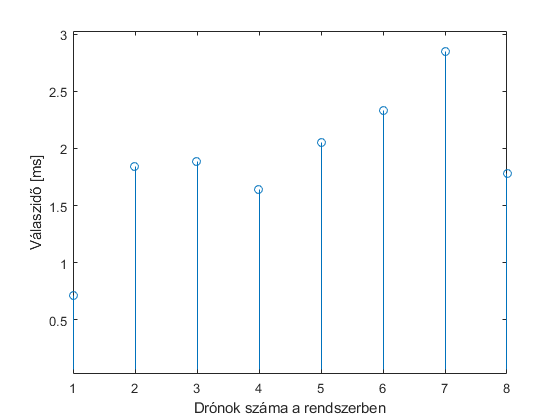
\includegraphics{figures/meres_ping.png}
	\caption{Válaszidő a drónok számának függvényében}
	\label{fig:meresping}
\end{figure}

\noindent
A válaszidőt 25 ICMP ping visszaérkezési idők átlagaként számoltam ki, úgy hogy a drón virtuális konténeréből küldtem a Roscore konténer interfészére. Az eredményen az látszik, hogy nő az üzemeltetett konténerek függvényében a válaszidő, nem drasztikusan, azonban valamilyen lineáris görbére illeszthetően (\ref{fig:meresping}. ábra).  \\

\begin{figure}
	\centering
	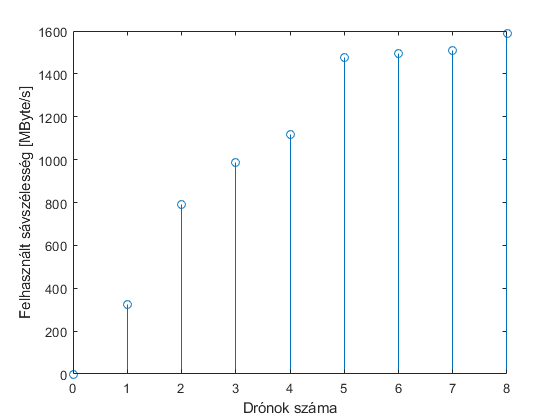
\includegraphics{figures/meres_iperf_inv.png}
	\caption{Felhasznált sávszélesség a drónok számának függvényében}
	\label{fig:meresiperf}
\end{figure}

\noindent
A sávszélességet \emph{iperf3} programmal néztem, szintén egy drón konténer és a hozzá tartozó Roscore között. A sávszélesség csökkenése is észrevehető, ugyan nincs mögötte az a linearitás, mint a válaszidő növekedésében, egy drónhoz képest megfeleződött a rendelkezésre álló kiszolgáltatott sávszélesség a klaszter felől. Az \emph{iperf3} program a rendelkezésre álló szabad sávszélességet mutatja meg, melyet teljes terhelés alatt mér meg egy rövid időablakban. Alaphelyzetben, egyetlen drón kapcsolatba lépése nélkül a két konténer között $f_{0}=2430 MB/s$-ot mértem a hálózat terhelésével. Ez azt jelenti, hogy drón kommunikáció nélkül ennyivel terhelhető a hálózat a két konténer között, amelyet a hardver és a virtualizáció határoz meg. Ez $f_0$ kezdeti értékre és kiszámított $x$ függvény pontjaira illeszthető görbe a GeoAlgebra függvényillesztő segítségével \[ x(n) = 625 \cdot ln(7.28n) [MB/s]\] eredmény jött ki, ahol $n$ a rendszerben lévő drónok száma. Egy felhasználási ábrát rajzoltattam ki, amely azt mutatja, hogy a kommunikáció nélküli elérhető sávszélességhez képest mennyi sávszélességet használnak a drónok, tehát: \[x_n = | f_n - f_0 |\] E mellé kimértem tcpdump-al egy félperces időablakban a drón és üzenetváltását a Roscore-al, amiből kijött, hogy n=1-re $\mu = 46.73 kérés/s$. Amiből kijön a kiszolgálási idő: \[\lambda= \mu-\frac{1}{D_1} = 46.73-\frac{1}{0.241} = 42.58 s \] Kiszámítottam a kiszolgálási időből és a kérési intenzitásból a késleltetés többi értékét a modell alapján a $D_1$ értékre vetítve és a mért értékek mellé vetettem (\ref{fig:meresiperf}. ábra)  \\

\begin{figure}
	\centering
	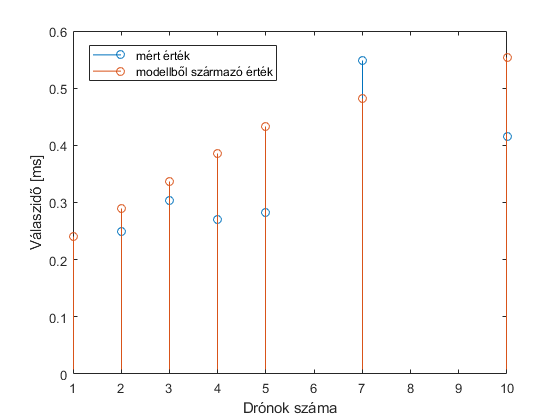
\includegraphics{figures/meres_iperf_model.png}
	\caption{Kiszolgálási válaszidő a drónflotta méretének függvényében}
	\label{fig:meresros}
\end{figure}

\noindent
Az \ref{cha:toki} fejezetben vizsgáltuk a matematikai modelljét egy M/M/1 kiszolgálási Erlang rendszernek. A diplomatervezés folyamatában a ROS rendszernek a megismerése közben kiderült, hogy a jelenlegi irányító szoftver arra nincs felkészítve, hogy egy Roscore-on keresztül irányítson több drónt, illetve az általam megalkotott végső Kubernetes rendszerben minden drónnak külön Roscore-ja van. Azért megnézzük, hogy mi lenne akkor ha lenne egy ROS-on keresztül N résztvevőjű flottát irányító szoftverünk, amely egy Roscore-on keresztül vezérelné a flottát. A mérést egy drón konténere és az egyetlen Roscore között végeztem a felhőben. A tiszta mérés kedvéért nem deploy-oltam az irányításra és kamerafeldolgozásra szolgáló konténereket. Egy és tizenöt drón között mértem a válaszidőt a ping programmal, 25 visszapattanást átlagolva (\ref{fig:meresros}. ábra). Jól látszik, hogy növekszik a drónok növelésével az egy drón felé lehetséges kiszolgálási idő. Tehát növekszik az \ref{cha:toki}. fejezetben megmutatott $\mu$ érték, amely fordítottan arányos a késleltetéssel.

\section{Késleltetés hozadéka 5G közeghozzáférés esetén}
A mérésekben megnéztük, hogy milyen késleltetések és sávszélességek vannak egy teljesen virtualizált rendszerben. Egy valós hálózaton és fizikai drónnal működő rendszerrel még hozzájön két rendszerből származó érték ezekhez a késleltetésekhez és sávszélességekhez. Értelemszerűen a késleltetéshez hozzáadódik, a sávszélességnél pedig az értékek minimumára csökken. \\

\noindent
A hálózat késleltetése és a közeghozzáférési technológia késleltetése adódik hozzá a teljes válaszidőhöz. A tanszéken kipróbált Wifi-s közeghozzáférés körülbelül $300 ms$-ot növel a szimulációhoz képest. Az 5G $5-15 ms$ körüli értéket is biztosíthat, így ezzel a technológiával minimalizálni lehet a teljes késleltetést az előző pontban kiszámoltakhoz konvergálva.
\chapter{Válaszidő 5G-s közeghozzáférési technológiával}
\addcontentsline{toc}{chapter}{Összegzés}
\chapter*{Összegzés}
A dolgozatban megnéztem mire hasznának ma tömeges robotos irányítást, specifikusabban kitekintettünk, hogy mely iparágakban használhatóak a drónok, mire és hogyan használják. Megnéztem mire jó a konténerizáció, elmerültünk a konténer alapú felhőrendszerek világában, összehasonlítottuk a Docker Swarm-ot, a Mesos-t és a Kubernetest. Átnéztem a robot- és drónirányítással kapcsolatos szoftvereket, hogy mik a lehetőségek, hogyan és minek szükséges jól együttműködni egy fizikai vagy egy szimulált drón irányításához. Megnéztem, hogyan lehet nagyobb számú drónt szimulálni. Megvalósítottam két tesztet, konténerekkel való drónirányítás és jelfeldolgozás tesztjét és különböző VM-ekről drónszimulálás tesztet. Továbbá megnéztem, hogyan tudjuk megbecsülni nagyszámú drónkiszolgálásnak a késleltetését. Elkészítettem egy automatikusan felépülő virtuális Kubernetes rendszert. Ezen rendszeren teszteltem a Kubernetes API széles palettáján több drónvezérlési architektúrát. Definiáltam egy QoS feltételrendszert, majd kiválasztottam és módosítottam azt az architektúrát amely ennek a legjobban megfelel. Megterveztem és implementáltam egy kiegészítőszoftvert, amely folyamatosan figyeli a kapcsolatot a drón és a felhőrendszer között, amennyiben tud javítani a kapcsolaton ezt megteszi, ha kritikus állapotba lép és nem tud javítani, akkor pedig figyelmezteti a felhasználót. Implementáltam egy algoritmust, amely a távoli drónvezérlés során szükséges videó folyamok és vezérlési adatok együttes minőségbiztosítását végzi. Méréseket végeztem a különböző részfeladatokról és terheltségről.


% Acknowledgements
%~~~~~~~~~~~~~~~~~~~~~~~~~~~~~~~~~~~~~~~~~~~~~~~~~~~~~~~~~~~~~~~~~~~~~~~~~~~~~~~~~~~~~~
%%----------------------------------------------------------------------------
\chapter*{\koszonetnyilvanitas}\addcontentsline{toc}{chapter}{\koszonetnyilvanitas}
%----------------------------------------------------------------------------

Ez nem kötelező, akár törölhető is. Ha a szerző szükségét érzi, itt lehet köszönetet nyilvánítani azoknak, akik hozzájárultak munkájukkal ahhoz, hogy a hallgató a szakdolgozatban vagy diplomamunkában leírt feladatokat sikeresen elvégezze. A konzulensnek való köszönetnyilvánítás sem kötelező, a konzulensnek hivatalosan is dolga, hogy a hallgatót konzultálja.


% List of Figures, Tables
%~~~~~~~~~~~~~~~~~~~~~~~~~~~~~~~~~~~~~~~~~~~~~~~~~~~~~~~~~~~~~~~~~~~~~~~~~~~~~~~~~~~~~~
%\listoffigures\addcontentsline{toc}{chapter}{\listfigurename}
%\listoftables\addcontentsline{toc}{chapter}{\listtablename}
%\lstlistoflistings\addcontentsline{toc}{chapter}{\lstlistlistingname}

% Bibliography
%~~~~~~~~~~~~~~~~~~~~~~~~~~~~~~~~~~~~~~~~~~~~~~~~~~~~~~~~~~~~~~~~~~~~~~~~~~~~~~~~~~~~~~
\addcontentsline{toc}{chapter}{\bibname}
\bibliography{bib/mybib}


% Appendix
%~~~~~~~~~~~~~~~~~~~~~~~~~~~~~~~~~~~~~~~~~~~~~~~~~~~~~~~~~~~~~~~~~~~~~~~~~~~~~~~~~~~~~~
%%----------------------------------------------------------------------------
\appendix
%----------------------------------------------------------------------------
\chapter*{\fuggelek}\addcontentsline{toc}{chapter}{\fuggelek}
\setcounter{chapter}{\appendixnumber}
%\setcounter{equation}{0} % a fofejezet-szamlalo az angol ABC 6. betuje (F) lesz
\numberwithin{equation}{section}
\numberwithin{figure}{section}
\numberwithin{lstlisting}{section}
%\numberwithin{tabular}{section}

%----------------------------------------------------------------------------
\section{A TeXstudio felülete}
%----------------------------------------------------------------------------
\begin{figure}[!ht]
\centering
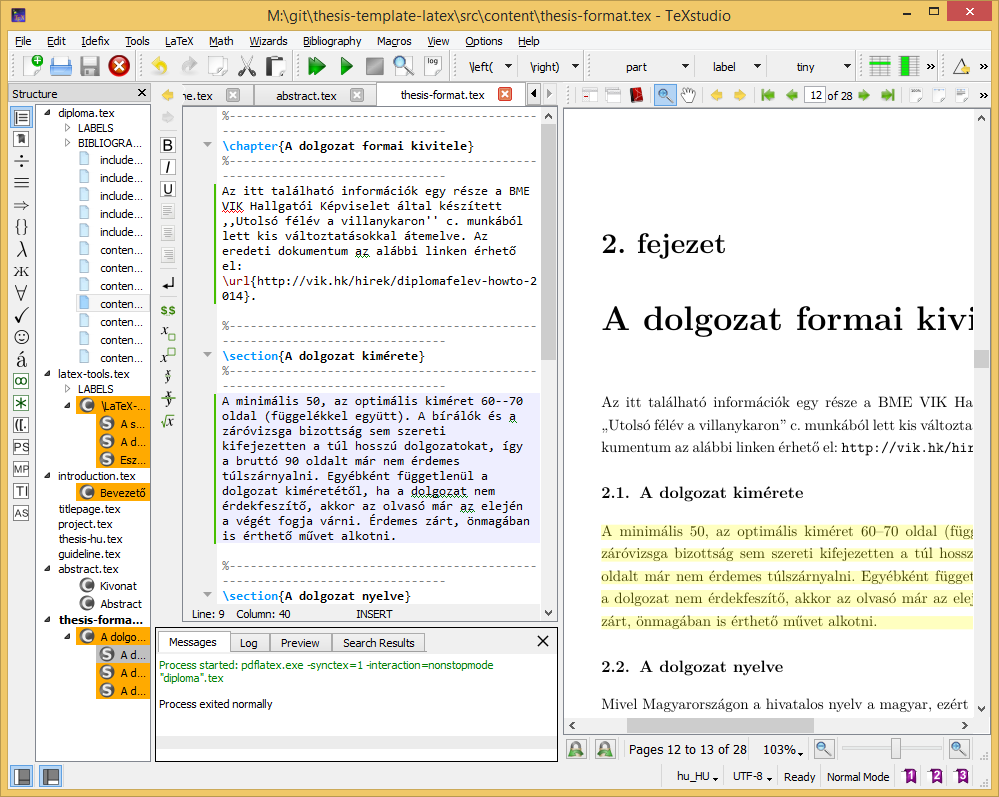
\includegraphics[width=150mm, keepaspectratio]{figures/TeXstudio.png}
\caption{A TeXstudio \LaTeX-szerkesztő.} 
\end{figure}

%----------------------------------------------------------------------------
\clearpage\section{Válasz az ,,Élet, a világmindenség, meg minden'' kérdésére}
%----------------------------------------------------------------------------
A Pitagorasz-tételből levezetve
\begin{align}
c^2=a^2+b^2=42.
\end{align}
A Faraday-indukciós törvényből levezetve
\begin{align}
\rot E=-\frac{dB}{dt}\hspace{1cm}\longrightarrow \hspace{1cm}
U_i=\oint\limits_\mathbf{L}{\mathbf{E}\mathbf{dl}}=-\frac{d}{dt}\int\limits_A{\mathbf{B}\mathbf{da}}=42.
\end{align}


%\label{page:last}
\end{document}
